\documentclass[a4paper,UKenglish]{lipics-v2018}

\usepackage{microtype}
\usepackage{xspace}
\usepackage{wrapfig}
\usepackage{stmaryrd}
\usepackage{xparse}
\usepackage{etoolbox}
\usepackage{mathpartir}
\usepackage{epigraph}
\setlength{\epigraphrule}{0pt}
\renewcommand*{\textflush}{flushright}
\setlength{\epigraphwidth}{4in}

\DeclareDocumentCommand\TR{om}{\EM{\IfNoValueTF{#1}{\PackageWarning{}{Undefined Type System}}{#1}\llbracket #2 \rrbracket}}

\DeclareDocumentCommand\TRG{omm}{\EM{\IfNoValueTF{#1}{\PackageWarning{}{Undefined Type System}}{#1}\llbracket #2 \rrbracket_{#3}}}
\DeclareDocumentCommand\TAG{ommm}{\EM{\IfNoValueTF{#1}{\PackageWarning{}{Undefined Type System}}{#1}\llparenthesis #2 \rrparenthesis_{#3}^{#4}}}
\newcommand{\OTS}{{\mathcal{O}}}
\newcommand{\CTS}{{\mathcal{C}}}
\newcommand{\BTS}{{\mathcal{B}}}
\newcommand{\TTS}{{\mathcal{T}}}
\newcommand{\SOMS}{{\mathcal{S}}}
\newcommand{\sspce}{;~}
\newcommand{\bscast}[2]{\EM{\BehCast{#1}{{#2}}}}
\newcommand{\WHERE}{~\EM{\xt{\bf where}}~}
\newcommand{\IF}{\EM{~\xt{\bf if}}~}
\newcommand{\HS}{\hspace{.2cm}}
\newcommand{\TypeCk}[3]{\EM{#1\vdash #2:#3}}
\newcommand{\EM}[1]{\ensuremath{#1}\xspace}
\newcommand{\xt}[1]{{\sf{#1}}}
\newcommand{\bt}[1]{\xt{\bf #1}}
\newcommand{\EMxt}[1]{\EM{\xt{#1}}}
\newcommand{\x}{\EMxt x}
\newcommand{\n}{\EMxt n}
\newcommand{\m}{\EMxt m}
\renewcommand{\mp} {\EMxt{m'}}
\newcommand{\s}{\EM{\sigma}}
\DeclareDocumentCommand\a{o}{\IfNoValueTF{#1}{\EMxt {a}}{\EM{\xt {a}_{#1}}}}
\DeclareDocumentCommand\ap{o}{\IfNoValueTF{#1}{\EMxt {a'}}{\EM{\xt {a'}_{#1}}}}
\DeclareDocumentCommand\app{o}{\IfNoValueTF{#1}{\EMxt {a''}}{\EM{\xt {a''}_{#1}}}}
\DeclareDocumentCommand\t{o}{\IfNoValueTF{#1}{\EMxt t}{\EM{\xt t_{#1}}}}
\DeclareDocumentCommand{\tp}{o}{\IfNoValueTF{#1}{\EM{ \xt t' }}{\EM{\xt t_{#1}'}}}
\DeclareDocumentCommand{\tpp}{o}{\IfNoValueTF{#1}{\EM{ \xt t'' }}{\EM{\xt t_{#1}''}}}
\DeclareDocumentCommand{\tppp}{o}{\IfNoValueTF{#1}{\EM{ \xt t''' }}{\EM{\xt t_{#1}'''}}}
\DeclareDocumentCommand{\e}{o}{\IfNoValueTF{#1}{\EM{ \xt e }}{\EM{\xt e_{#1}}}}
\DeclareDocumentCommand{\ep}{o}{\IfNoValueTF{#1}{\EM{ \xt e' }}{\EM{\xt e_{#1}'}}}
\DeclareDocumentCommand{\epp}{o}{\IfNoValueTF{#1}{\EM{ \xt e'' }}{\EM{\xt e''_{#1}}}}
\DeclareDocumentCommand{\eppp}{o}{\IfNoValueTF{#1}{\EM{ \xt e''' }}{\EM{\xt e'''_{#1}}}}
\DeclareDocumentCommand{\fd}{o}{\IfNoValueTF{#1}{\EM{ \xt{fd} }}{\EM{\xt{fd}_{#1}}}}
\DeclareDocumentCommand{\fdp}{o}{\IfNoValueTF{#1}{\EM{ \xt{fd}' }}{\EM{\xt{fd}_{#1}'}}}
\DeclareDocumentCommand{\fdpp}{o}{\IfNoValueTF{#1}{\EM{ \xt{fd}'' }}{\EM{\xt{fd}_{#1}''}}}
\DeclareDocumentCommand{\fdppp}{o}{\IfNoValueTF{#1}{\EM{ \xt{fd}''' }}{\EM{\xt{fd}_{#1}'''}}}
\DeclareDocumentCommand{\md}{o}{\IfNoValueTF{#1}{\EM{ \xt{md} }}{\EM{\xt{md}_{#1}}}}
\DeclareDocumentCommand{\f}{o}{\IfNoValueTF{#1}{\EM{ \xt f }}{\EM{\xt f_{#1}}}}
\DeclareDocumentCommand{\mdp}{o}{\IfNoValueTF{#1}{\EM{ \xt{md}' }}{\EM{\xt{md}_{#1}'}}}
\DeclareDocumentCommand{\mdpp}{o}{\IfNoValueTF{#1}{\EM{ \xt{md}'' }}{\EM{\xt{md}_{#1}''}}}
\DeclareDocumentCommand{\mdppp}{o}{\IfNoValueTF{#1}{\EM{ \xt{md}''' }}{\EM{\xt{md}_{#1}'''}}}
\DeclareDocumentCommand{\C}{o}{\IfNoValueTF{#1}{\EM{ \xt{C} }}{\EM{\xt{C}_{#1}}}}
\DeclareDocumentCommand{\mt}{o}{\IfNoValueTF{#1}{\EM{ \xt{mt} }}{\EM{\xt{mt}_{#1}}}}
\DeclareDocumentCommand{\mtp}{o}{\IfNoValueTF{#1}{\EM{ \xt{mt}' }}{\EM{\xt{mt}_{#1}'}}}
\DeclareDocumentCommand{\mtpp}{o}{\IfNoValueTF{#1}{\EM{ \xt{mt}'' }}{\EM{\xt{mt}_{#1}''}}}
\DeclareDocumentCommand{\mtppp}{o}{\IfNoValueTF{#1}{\EM{ \xt{mt}''' }}{\EM{\xt{mt}_{#1}'''}}}
\DeclareDocumentCommand{\D}{o}{\IfNoValueTF{#1}{\EM{ \xt{D} }}{\EM{\xt{D}_{#1}}}}
\DeclareDocumentCommand{\Dp}{o}{\IfNoValueTF{#1}{\EM{ \xt{D'} }}{\EM{\xt{D'}_{#1}}}}
\DeclareDocumentCommand{\Dpp}{o}{\IfNoValueTF{#1}{\EM{ \xt{D''} }}{\EM{\xt{D''}_{#1}}}}
\newcommand{\K}{\EMxt K}
\renewcommand{\k} {\EMxt k}
\newcommand{\Kp}{{\EMxt{K'}}}
\renewcommand{\sp}{{{\EM{\s'}}}}
\newcommand{\A}{\EMxt {A}}
\newcommand{\I}{\EMxt {I}}
\newcommand{\E}{\EMxt {E}}
\newcommand{\Cp}{\EMxt{C'}}
\newcommand{\M}{\EMxt{M}}
\newcommand{\Env}{\EM{\Gamma}}
\newcommand{\EE}{\EM{\textsf{{E}}}}
\newcommand{\any}{\EM{\star}}
\newcommand{\this}{\EMxt{this}}
\newcommand{\that}{\EMxt{that}}
\newcommand{\FRead}[1]{\EM{\this.#1}}
\newcommand{\FWrite}[2]{\EM{\this.#1} = #2}
\newcommand{\FReadR}[2]{\EM{#1.#2}}
\newcommand{\FWriteR}[3]{\EM{#1.#2} = #3}
\newcommand{\Call}[3]{\EM{#1.#2(#3)}}
\newcommand{\KCall}[5]{\EM{{#1}.{#2}_{{#4} \shortrightarrow {#5}}(#3)}}
\newcommand{\DynCall}[3]{\EM{#1@#2_{\any\shortrightarrow\any}(#3)}}
\newcommand{\New}[2]{\EM{\new\;#1(#2)}}
\newcommand{\SubCast}[2]{\EM{\langle{#1}\rangle\,{#2}}}
\newcommand{\BehStart}{\EM{\blacktriangleleft}}
\newcommand{\BehEnd}{\EM{\blacktriangleright}}
\newcommand{\BehCast}[2]{\EM{\BehStart\! #1\! \BehEnd #2}}
\newcommand{\new}{\EM{\bt{new}}}
\newcommand{\HT}[2]{\EM{{#1}\!:{#2}}}
\newcommand{\Mdef}[5]{\EM{ \HT{ #1( \HT{#2}{#3})}{#4}\;\{{#5}\}}}
\newcommand{\obj}[2]{ \EM{ #1\{#2\}}}
\newcommand{\behcast}[7]{\EM{#5\,#6\,#7 = \xt{bcast}(#1, #2, #3, #4)}}
\newcommand{\behcastE}[7]{\EM{\xt{bcast}(#1, #2, #3, #4) = #5\,#6\,#7}}
\newcommand{\behcastS}[4]{\EM{\xt{bcast}(#1, #2, #3, #4)}}
\newcommand{\B}{\EM{~|~}}
\newcommand{\Red}{\EM{\rightarrow}}
\newcommand{\class}{\EM{\bf{class}}}
\newcommand{\Class}[3]{\EM{\bt{class}\;#1\,\{\,#2~#3\,\}}}
\newcommand{\Ftype}[2]{\EM{ \HT{#1}{#2} }}
\newcommand{\Fdef}[2]{\EM{ \HT{#1}{#2} }}
\newcommand{\Mtype}[3]{\EM{ \HT{#1(#2)}{#3}}}
\newcommand{\Map}[2]{\EM{ #1[#2] }}
\newcommand{\Bind}[2]{\EM{#1 \mapsto #2}}
\newcommand{\Sub}{\EM{<:}}
\newcommand{\OK}{\EM{~\checkmark}}
\newcommand{\names}[1]{\EM{\xt{names}(#1)}}
\newcommand{\cload}[1]{\EM{\xt{nodups}(#1)}}
\newcommand{\EnvType}[5]{ \EM{#1\,#2\,#3\vdash #4 : #5}}
\newcommand{\Rule}[4][]{\inferrule*{#3}{#4}}
\newcommand{\HasType}[3]{ \EM{#1} (\EM{#2}) = \EM{#3}}
\newcommand{\wrap}[4]{\EM{\xt{W}(#1,#2,#3,#4)}}
\newcommand{\wrapAny}[3]{\EM{\xt{W}\!\any(#1,#2,#3)}}
\newcommand{\ConvertE}[4]{\EM{#1 \vdash_{\!s} #3 \Mapsto #4}}
\newcommand{\In}{\EM{\in}}
\newcommand{\App}[2]{\EM{#1(#2)}}
\newcommand{\SSub}[4]{\EM{#1~#2\vdash_{\!s} #3\Sub #4}}
\newcommand{\StrSub}[4]{\EM{#1~#2\vdash #3\Sub #4}}
\newcommand{\EnvTypeS}[4]{ \EM{#1\,#2\vdash_{\!s} #3 : #4}}
\newcommand{\WFp}[2]{#1~#2\OK}
\newcommand{\WFq}[1]{#1\OK}
\newcommand{\fresh}[1]{\EM{#1~\xt{fresh}}}
\newcommand{\figref}[1]{Fig.~\ref{#1}\xspace}
\newcommand{\kafka}{{\sf KafKa}\xspace}
\newcommand{\src}[1]{\colorbox[gray]{0.89}{$#1$}}

\definecolor{kgray}{gray}{0.89}
\newcolumntype{k}{>{\columncolor{kgray}}r}

\newcolumntype{E}{>{\ttfamily}l<{}@{}}
\newcolumntype{V}{>{\hspace{1mm}\begin{minipage}{4.3cm}}l<{\end{minipage}\hspace{1mm}}@{}}
\newcolumntype{R}[1]{>{\hspace{1mm}\begin{minipage}{#1}}l<{\end{minipage}\hspace{1mm}}@{}}

\newcounter{rules}
\newenvironment{rules}[2]{\vspace{0.5em}\ebox{#2}
\vspace{-1.5em}\setlength{\parskip}{2em}
\renewenvironment{rule}[1]{\protected@edef\@currentlabel{\textsc{#1-##1}}
\RightLabel{(\textsc{#1-##1})}
}{}
}{\vspace{1em}}

\newcounter{theo}
\renewcommand{\thetheo}{\textbf{\arabic{theo}}}

\newcounter{lem}
\renewcommand{\thelem}{\textbf{\arabic{lem}}}

\newcounter{conds}
\newbool{condonce}
\newcounter{cond}[conds]
\renewcommand{\thecond}{\textbf{\alph{cond}}}
\newenvironment{conds}
{\textit{\ifbool{condonce}{and if:}{If:\booltrue{condonce}}}
\renewcommand{\cond}[1]{\par\hspace{2em}\numbox{cond}{\thecond}##1}}{}
\newcommand{\cond}[1]{\begin{conds}\cond{#1}\end{conds}}

\newenvironment{analysis}[1]
{\vspace{.5em} \textbf{Case analysis} on #1\par

\renewcommand{\thestep}{\textbf{\roman{step}}}}{}
\newcommand{\stepwidth}{.55\textwidth-\leftskip}
\newcommand{\numwidth}{3.5em}
\newcommand{\numbox}[2]{\refstepcounter{#1}\makebox[\numwidth][l]{#2.}}
\newcommand{\stepnum}{\numbox{step}{\thestep}}

\newbool{stepspace}
\newcommand{\stepspace}{\ifbool{stepspace}{\vspace{0.4em}\boolfalse{stepspace}}{}\par}
\newcommand{\step}[2]{\stepspace\par\stepnum\makebox[\stepwidth][l]{#1} by #2}

\newsavebox{\stepsby}
\newenvironment{steps}[1]
{\savebox{\stepsby}{#1}
\renewcommand{\step}[1] {\stepnum##1\par}\stepspace
\begin{math}\left.\hspace{-.1em}\begin{minipage}{\numwidth+\stepwidth}}
{ \end{minipage}\right\}\end{math} by \usebox{\stepsby}\par}

\newenvironment{longsteps}[1]
{
\newcommand{\stepsbysavedvalue}{#1}
\renewcommand{\step}[1] {\stepnum##1\par}\stepspace
\begin{math}\left.\hspace{-.1em}\begin{minipage}{\numwidth+\stepwidth}}
{ \end{minipage}\right\}\end{math} \begin{minipage}{\textwidth-\stepwidth+1em}by \stepsbysavedvalue{}\end{minipage}\par}

\ProvidesFile{omscmtt.fd}
\DeclareFontFamily{OMS}{cmtt}{\skewchar\font48 }
\DeclareFontShape{OMS}{cmtt}{m}{n}{<->ssub*cmsy/m/n}{}
\DeclareFontShape{OMS}{cmtt}{m}{it}{<->ssub*cmsy/m/n}{}
\DeclareFontShape{OMS}{cmtt}{m}{sl}{<->ssub*cmsy/m/n}{}
\DeclareFontShape{OMS}{cmtt}{m}{sc}{<->ssub*cmsy/m/n}{}
\DeclareFontShape{OMS}{cmtt}{bx}{n}{<->ssub*cmsy/b/n}{}
\DeclareFontShape{OMS}{cmtt}{bx}{it}{<->ssub*cmsy/b/n}{}
\DeclareFontShape{OMS}{cmtt}{bx}{sl}{<->ssub*cmsy/b/n}{}
\DeclareFontShape{OMS}{cmtt}{bx}{sc}{<->ssub*cmsy/b/n}{}

\definecolor{Gray}{gray}{0.9}
\definecolor{vlightgray}{gray}{0.93}

\nolinenumbers
\lstdefinelanguage{JavaScript}{
keywords={typeof,new,true,false,instanceof,catch,function,return,null, 
catch, switch, var, if, in, while, do, else, case, break},
keywordstyle=\color{darkgray},
ndkeywords={class,def,interface,export,boolean,throw,extends,implements,import,this},
ndkeywordstyle=\color{darkgray}\bfseries,
identifierstyle=\color{black},
sensitive=false, comment=[l]{//}, morecomment=[s]{/*}{*/},
commentstyle=\color{gray}\ttfamily, stringstyle=\color{gray}\ttfamily,
morestring=[b]', morestring=[b]",
aboveskip=\medskipamount, belowskip=\medskipamount, escapeinside={(*@}{@*)}
}
\lstset{
language=JavaScript, extendedchars=true, basicstyle=\small\ttfamily,
showstringspaces=false, showspaces=false, numberstyle=\small,
numbersep=9pt, tabsize=2, breaklines=true, showtabs=false, captionpos=b
}

\newcommand{\rot}[1]{\rotatebox{80}{#1}\hspace{-10px}}
\newcommand{\X}{\EM{\bullet}}
\newcommand{\XX}{\EM{\bullet^{2}}}
\newcommand{\XY}{\EM{\bullet^{1}}}
\newcommand{\Int}{\xt{Int}}
\newcommand{\W}{\xt{W}\xspace}

\title{KafKa: Gradual Typing for Objects}
\titlerunning{Gradual Typing for Objects}

\author{Benjamin Chung}{Northeastern University, Boston, MA, USA}{}{}{}
\author{Paley Li}{Czech Technical University, Prague, Czech Republic, and \\Northeastern University, Boston, MA, USA}{}{}{}
\author{Francesco Zappa Nardelli}{INRIA, Paris, France}{}{}{}
\author{Jan Vitek}{Czech Technical University, Prague, Czech Republic, and \\Northeastern University, Boston, MA, USA}{}{}{}


\authorrunning{B. Chung, P. Li, F. Zappa Nardelli, and J. Vitek}
\Copyright{Benjamin Chung, Paley Li, Francesco Zappa Nardelli, and Jan Vitek}
\subjclass{\ccsdesc{Software and its engineering~Semantics}}
\keywords{Gradual typing, object-orientation, language design, type systems}
\acknowledgements{The author thank the reviewers of {\sc ecoop},
{\sc popl}, {\sc esop}, and again {\sc ecoop} for comments that gradually
improved this paper. We are grateful to Leif Andersen, Fabian Muelbrock, Éric Tanter, Celeste Hollenbeck, Sam Caldwell, Ming-Ho Yee, Lionel Zoubritzky, Benjamin Greenman and
Matthias Felleisen for their feedback.}
\funding{This work received funding from the European
Research Council (ERC) under the European Union’s Horizon 2020 research and
innovation programme (grant agreement 695412), the NSF (award 1544542 and
award 1518844) as well as ONR (award 503353).}


\supplement{ECOOP Artifact Evaluation approved artifact available at\\ \url{http://dx.doi.org/10.4230/DARTS.4.3.10}}


\EventEditors{Todd Millstein}
\EventNoEds{1}
\EventLongTitle{32nd European Conference on Object-Oriented Programming (ECOOP 2018)}
\EventShortTitle{ECOOP 2018}
\EventAcronym{ECOOP}
\EventYear{2018}
\EventDate{July 16--21, 2018}
\EventLocation{Amsterdam, Netherlands}
\EventLogo{aec-badge-ecoop}
\SeriesVolume{109}
\ArticleNo{12}

\begin{document}

\maketitle

\begin{abstract} 
A wide range of gradual type systems have been proposed, providing many
languages with the ability to mix typed and untyped code. However, hiding
under language details, these gradual type systems embody fundamentally
different ideas of what it means to be well-typed. In this paper, we show that
four of the most common gradual type systems provide distinct guarantees,
and we give a formal framework for comparing gradual type systems for
object-oriented languages. First, we show that the different gradual type
systems are practically distinguishable via a three-part litmus test. 
We present a formal framework for defining and comparing gradual type
systems. Within this framework, different gradual type systems become
translations between a common source and target language, allowing for
direct comparison of semantics and guarantees.
\end{abstract}

\section{Introduction}

\epigraph{\small\vspace{-4mm}
\it ``Because half the problem is seeing the problem''}

\vspace{-7mm}\noindent There never was a single approach to gradual
typing. The field was opened by two simultaneously published papers. One, by
Siek and Taha, typed individual Scheme terms using a consistency relation,
casts being inserted by a type directed translation~\cite{SiekTaha06}. The
other, by Tobin-Hochtstadt and Felleisen, described a system allowing
programmers to add types to individual modules, using constraint solving to
determine where contracts are needed to protect typed and untyped code from
each other~\cite{tf-dls06}. These two approaches set the tone for a decade
of research. Today, gradual type systems rely on a variety of languages,
enforcement mechanisms with various guarantees; this linguistic diversity is
not without consequence, however, as the very notion of what constitutes an
error remains unsettled.

The type system and semantics of a programming language are necessarily
tightly coupled; each has to deal with the language's complexity. As a
result, the same gradual type system may seem very different when applied to
two different languages, an issue that shows up clearly with object-oriented
languages. Siek and Taha's first effort~\cite{SiekTaha07} presented a
gradual type system for an object-oriented programing language. It related objects by generalizing
the notion of consistency~\cite{SiekTaha06} over structural subtyping. The
work had drawbacks, most notably in the handling of mutable state and
aliasing -- vital features of object-oriented languages. Underlying each
subsequent gradual type system are different design choices on how to deal
with mutability and aliasing.

The landscape of gradually typed object-oriented languages is rich and includes:\medskip
\begin{itemize}
\item Typed Racket: a rich gradual type system based on contracts.
\item Gradualtalk: a gradual variant of Smalltalk.
\item C\#: a statically typed language with a dynamic type.
\item Dart: a class-based language with optional types.
\item Hack: a statically typed variant of PHP that allows untyped code.
\item Thorn: a language with both statically typed and untyped code.
\item TypeScript: JavaScript with optional types.
\item StrongScript: a variant of TypeScript with nominal types.
\item Nom: a language supporting dynamic types and nominal typing.
\item Reticulated Python: a family of gradual type systems for Python.
\end{itemize}
\medskip These languages differ in their type systems and associated
run-time enforcement strategies. There are four major approaches, labeled here
as optional, concrete, behavioral, and transient. The \emph{optional}
approach, chosen by TypeScript, Dart, and Hack, amounts to static
type checking followed by type erasure. Erroneous values flowing from
dynamically typed code to statically typed code will not be caught. The
\emph{concrete} approach, used in C\# and Nom, uses run-time subtype tests
on type constructors to supplement static typing. While statically typed
code executes at native speed, values are dynamically checked at
typed-untyped boundaries. The \emph{behavioral} approach of Typed Racket and
Gradualtalk monitors values to ensure that they behave in accordance to
their assigned types. Instead of checking higher-order and mutable values
for static type tags like concrete, wrappers ensure enduring conformance of
values to their declared type. The \emph{transient} approach, specific to
Reticulated Python, lies between concrete and behavioral; it adds type casts
but does so only for the top level of data structures. Finally, Thorn and
StrongScript combine the optional and concrete approaches, differentiating
between erased types and run-time-checked types.

Static type systems for object-oriented languages are designed to prevent dynamic ``method not understood'' errors. For
gradual type systems, however, some method not found errors cannot be ruled out before
execution. In such a gradual type system, untyped code can pass an ill-typed value to typed code, breaking soundness. 
The meaning of an ``error'' for a gradual type system, therefore, depends on how type specifications are
enforced. In other words, each gradual type system may catch different
``errors.'' We demonstrate this with a litmus test consisting of three
simple programs capable of distinguishing the four above-mentioned
approaches. The litmus test programs are statically well-typed and
``correct'' in the sense that they run to completion without error in an
untyped language. However, when executed under different gradual typing
systems, they produce different errors. For intuition, consider a call,
\EM{\x.\m()}, where \EM{\x:\C} and \C has a method \m returning a \D. In
the concrete approach, this call will succeed. With behavioral, the call
will go through, but an error may be reported if \m returns a value of the
wrong type. In transient, the call is similarly guaranteed to go through,
but might return the wrong type without reporting an error. Finally, in
optional, the call may get stuck, as \x may not have a method named \m; and,
if it succeeds, there is no guarantee that type \D will be returned.

\begin{wrapfigure}{r}{5cm}
\vspace{-6mm}
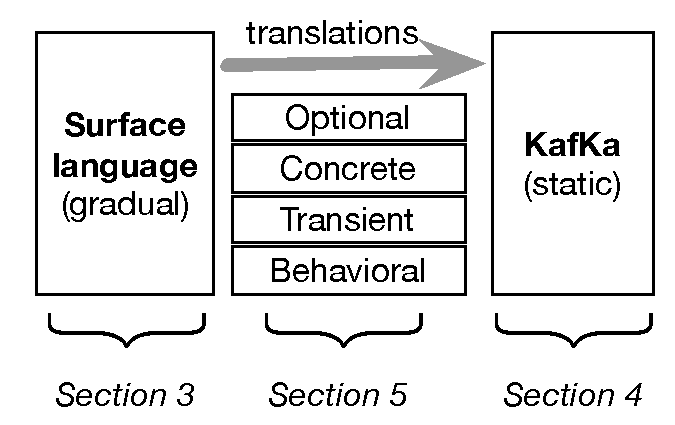
\includegraphics[width=5cm]{fig1}
\vspace{-8mm}\end{wrapfigure}

We propose to compare approaches to gradual typing for objects by
translating a gradually typed surface language to a target language called
\kafka. Our surface language is a \emph{gradually} typed class-based object-oriented 
language similar to Featherweight Java. \kafka is a
\emph{statically} typed class-based object calculus with mutable state. The
key difference between the two is the sound type system and casts of \kafka.
Where the surface language allows implicit coercions, \kafka requires
explicit casts to convert types. Casts come in two kinds: \emph{structural
casts} check for subtyping, while \emph{behavioral casts} monitor that an
object behaves as if it was of some type. Translating from surface to target
language involves adding casts, the location and type of which depends on
the gradual type system.

This paper makes the following contributions:\medskip
\begin{itemize} 
\item The design of a core calculus for gradual type systems for objects.
\item Translations of each gradual approach to the core calculus.
\item A litmus test comprised of three programs to tell apart the gradual
type systems.
\item Supplementary material includes a mechanized proof of soundness of the
type system of the core calculus and its proof-of-concept implementation
on .Net.
\end{itemize}
\medskip
Our work does not address the question of performance of the
translations. Each of the semantics for gradual typing has intrinsic
performance costs; but these can be mitigated by compiler and run-time
optimizations, which we do not perform. \kafka departs from prior work
(e.g.~\cite{greenman18} as \kafka is statically typed. By translating
to a statically typed core, we can clearly see where wrapper-induced dynamic
errors can occur. Another design choice is the use of structural subtyping
in \kafka. This is motivated by our desire to represent behavioral and
transient approaches that require structural subtyping. We do not foresee
difficulties either switching to a nominal type system or providing an
additional nominal subtype cast. Code and proofs are available from: {\small
\url{github.com/BenChung/GradualComparisonArtifact}.}

\section{Background}

\epigraph{\vspace{-4mm}\small\it ``If you know the enemy and know yourself...''}

\vspace{-7mm}
\noindent The intellectual lineage of gradual typing can be traced back to
attempts to add types to Smalltalk and LISP. On the Smalltalk side, work on
the Strongtalk optional type system~\cite{Bracha93} led to Bracha's notion
of pluggable types~\cite{pluggabletypes}. In Bracha's notion of pluggable types, types exist solely to
catch errors at compile-time, never affecting the run-time behavior of
programs. An optional type system is \emph{trace preserving}:
that is to say, if a term \e reduces to \a, then adding type annotations to
\e does not prevent it from reducing to \a~\cite{ecoop15}. This property is valuable to
developers as it ensures that type annotations will not introduce errors; and
thus, adding types does not increase the testing burden!
Optional type systems in wide use include Hack~\cite{hack13},
TypeScript~\cite{BAT14} and Dart~\cite{dart13}.

Felleisen and his students have contributed substantially to gradual
typing. The Typed Scheme~\cite{tf-popl08} design, that later became Typed
Racket, is influenced by their earlier work on higher-order
contracts and semantic casts~\cite{ff-icfp02,semanticasts}. 
Typed Racket was envisioned as a vehicle for
teaching programming, being able to explain the source of errors and
avoiding surprises for beginning users were important considerations. 
For this reason, a value that flowed in a variable of type \t, 
was required behave as if it belonged
to that type throughout its lifetime. Whenever a higher-order or mutable
value crosses a boundary between typed and untyped code, it is wrapped in a
contract that monitors the value's behavior. If the value misbehaves, blame
can be assigned to the boundary that assigned it the type that was
violated. The granularity of typing is the module, thus a module is either
entirely typed or entirely untyped. Typed Racket's support for objects was
described by Takikawa et al.~\cite{Takikawa:2012}.

Siek and Taha coined the term gradual typing in~\cite{SiekTaha06} as ``any
type system that allows programmers to control the degree of static checking
for a program by choosing to annotate function parameters with types, or
not.'' They formalized this idea in the lambda calculus augmented with
references. To make the type system a gradual one, they defined the type
consistency relation $\t \sim \tp$. If $\t \sim \tp$, then \t is consistent
with \tp, and can therefore be used implicitly where a \tp instance is
expected. This enables gradual typing, as $\any \sim \t$ for every $\t$ and
vice versa, allowing untyped values to be passed where typed ones are
expected. Siek and Taha extended this idea to an object
calculus~\cite{SiekTaha07}. 
In order to do so, they combined consistency with structural
subtyping, producing consistent subtyping. With consistent subtyping,
consistency can be used when checking structural subtyping, allowing typed
objects and untyped objects to be mixed. To explore the design space,
Reticulated Python~\cite{siek14} was given three modes: the \emph{guarded}
mode behaves as Typed Racket with contracts applied to values. The
\emph{transient} mode performs shallow subtype checks on reads and method
returns, only validating if the value obtained has matching method types.
The \emph{monotonic} mode is fundamentally different from any of the
previous approaches. Monotonic cast updates the type of values in place by
replacing some of the occurrences of \any with more specific types, and these
updates propagate recursively through the heap until fix-point.

Other noteworthy systems include Gradualtalk~\cite{GS13}, C\#
4.0~\cite{Bierman10}, Thorn~\cite{oopsla09}, Nom~\cite{Muehlboeck2017} and
Strong\-Script~\cite{ecoop15}. Gradualtalk is a variant of Smalltalk with
behavioral casts and mostly nominal type equivalence (structural equivalence
can be specified on demand, but it is rarely used). It has an optional mode
and a mode in which blame can be turned off. C\# 4.0 adds the type {\sf
dynamic} to C\# and adds dynamically resolved method invocation. Thus C\#
has a dynamic sublanguage that allows developers to write unchecked code,
working alongside a sound typed sublanguage in which values are always of
their declared type. The implementation replaces \any by the type {\tt
object} and adds casts where needed. Thorn and StrongScript extend the
C\# approach with the addition of optional types (called {\em like types} in
Thorn). Thorn is implemented by translation to the JVM. StrongScript
is implemented on top of a modified version of the V8 VM. The presence of concrete types means
that the compiler can optimize code (unbox data and in-line methods) and
programmers are ensured that type errors will not occur within concretely
typed code. Nom is similar to Thorn in that it is nominal and follows the
concrete approach.

\begin{figure}[!t]
\center
{\footnotesize
\begin{tabular}{r|lllllllllllllr}
& & \rot{Nominal}
& \rot{Optional}
& \rot{Concrete}
& \rot{Behavioral}
& \rot{Class based}
& \rot{First-class Class}
& \rot{Soundness claim}
& \rot{Unboxed prim.}
& \rot{Subtype cast}
& \rot{Shallow subtype cast}
& \rot{Behavioral cast}
& \rot{Blame}
& \rot{Pathologies}
\\
Dart &&\X &\X & & &\X & & & &\X & & & & - 
\\\hline
Hack &&\X &\X & & &\X & & & &\X & & & & - 
\\\hline
TypeScript && &\X & & &\X & & & & & & & & - 
\\\hline
C\# &&\X & &\X & &\X & &\XX & \X &\X & & &\X & - 
\\\hline
Thorn &&\X &\X &\X & &\X & &\XX & \X &\X & & & & -
\\\hline
StrongScript &&\X &\X &\X &\X &\X & &\XX & &\X & &\X & & 1.1x 
\\\hline
Nom 	 &&\X & &\X & &\X & &\XX & \X &\X & & &\X & 1.1x
\\\hline
Gradualtalk &&\XY& & &\X &\X & & \X & & & &\X &\X & 5x
\\\hline
Typed Racket && & & &\X &\X &\X &\X & & &\X &\X &\X & 121x 
\\\hline
Reticulated Python \\
\it Transient&& &\X & & & \X & & \X & & &\X & & & 10x \\
\it Monotonic&& & & &\X & \X & & \X & & & &\X & & 27x\\
\it Guarded && & & &\X & \X & & \X & & & &\X &\X & 21x\\
\end{tabular}}
\caption{Gradual type systems.~(1) Opt.~structural constraints.~(2)
Typed expressions are sound.}\label{over}
\end{figure}

\figref{over} reviews gradual type systems for objects. All languages are
class-based, except TypeScript which has both classes and JavaScript
objects. While that choice is not crucial; classes are useful as a source of
type declarations. Most languages build subtyping on explicit subtype
declarations, nominal typing, rather than on structural similarities.
TypeScript uses structural subtyping but does not implement a run-time
check for it. Anecdotal evidence suggests that TypeScript could switch
to nominal subtyping with little effort, as was done for
StrongScript~\cite{ecoop15}. While nominal subtyping leads to more
efficient type casts, Reticulated Python's subtype consistency relation is
fundamentally structural; it would be nonsensical to use it in a nominal
system. For Racket, the heavy use of first-class classes and class
generation naturally leads to structural subtyping as many of the classes
being manipulated have no names and arise during computation.

The optional approach is the default for Dart, Hack, and TypeScript.
Transient Reticulated Python allows any value to flow in a field, regardless
of type annotations, leading to its ``open world'' soundness
guarantee~\cite{siek14}. Some languages like Dart and Gradualtalk can
operate in a checked and an uncheck mode. In Thorn, Nom, and C\#, primitives
are concretely typed; they can be unboxed without tagging. The choice of
casts follows from other design decisions. The concrete approach naturally
tends to use subtype tests to establish the type of values. For nominal
systems, there are highly optimized algorithms. Shallow casts are casts that
only check the presence of methods but not their signature. They are used
by Racket and Reticulated Python to ensure some basic form of type
conformance. Behavioral casts are used when information, such as a type or a
blame label, must be associated with a reference or an object.

Blame assignment is a topic of investigation in its own right. Anecdotal
evidence suggests that the context provided by blame helps developers
pinpoint the provenance of errors. In the same way that a Java stack trace
identifies the function that went wrong, blame identifies where a type
assertion came from. This is especially important in behavioural gradual
type systems, as type assertions become wrappers which can propagate through
the heap. Blame identifies where a failing wrapper came from, a task that
would otherwise require extensive backtracking debugging. Unlike stack
traces, which have little run-time cost, blame tracking has a cost due to
its meta-data. Blame information has to be stored whenever a wrapper is
applied and is believed to cause substantial slowdowns. However, this has
not been measured in detail. With the concrete approach, blame is trivially
available as evaluation stops at the boundary that causes the
failure~\cite{Muehlboeck2017}. We are primarily concerned with where the
error arises, rather than what information is reported; thus, we
do not consider blame further.

The last column of \figref{over} lists self-reported performance
pathologies. These numbers are not comparable, as they refer to different
programs and different configurations of type annotations. They are not
worst case scenarios either; most languages lack a sufficient corpus of code
to conduct a thorough evaluation. Nevertheless, one can observe that for
optional types no overhead is expected, as the type annotations are erased
during compilation. Concrete types insert efficient casts and lead to code
that can be optimized. The performance of the transient semantics for
Reticulated Python is a worst case scenario for concrete types -- i.e, there
is a cast at almost every call. Finally, languages with behavioral casts are
prone to significant slowdowns. Compiler optimizations for reducing these
overheads are an active research
topic~\cite{OnlyMostly,richards-bettermono}. Languages such as C\#, Nom,
Thorn, and Strong\-Script are designed so that the performance of fully
typed code is better than untyped code, so that mixed code performs well
thanks to the relatively inexpensive nominal subtype tests.

In contemporary work, Greenman and Felleisen describe three approaches to
\emph{migratory typing} in the context of a lambda calculus extended with
pairs and primitive values~\cite{greenman18}. Their \emph{natural embedding}
corresponds to the behavioral approach, the \emph{erasure embedding} is the
optional approach, and the \emph{locally-defensive embeddeding} is
transient. They do not consider the concrete approach -- neither
objects or mutable state. They give performance results for a
non-optimizing implementation of the embeddedings, and the results are as
expected: behavioral has extreme worst cases and transient significantly
slows down fully-typed programs. While they do not evalute object-oriented
programs, these are unlikely to fare better. Our work differs in
that we are trying to express a translation between object calculi using
features that are readily available in most virtual machines.


\section{A Family of Gradually Typed Languages and their Litmus Test}\label{litmustest}

\epigraph{\vspace{-3mm}\small\it ``There is no perfection only life''} 

\vspace{-7mm}
\noindent
There is no single, common notion of what constitutes an erroneous gradually
typed program -- a consequence of the varied enforcement strategies. The choice
of enforcement strategy is reflected in the semantics of the language
which, in turn, implies that developers have to understand the details of
that strategy to avoid run-time errors. This also
means that it is possible to differentiate between approaches by simply
observing the run-time errors that each type system produces. We propose a
litmus test consisting of three programs whose execution depends on which
gradual type system is in use. Each of these programs is statically 
well-typed and runs without error when executed with a purely dynamic semantics.
However, this varies as we use different semantics for gradual typing.
We start by presenting a common surface language in which we can
express our programs, and then explain why the various approaches to gradual
typing yield different run-time errors.

\subsection{A Common Surface Language}

\begin{figure}[!t]\hrulefill \small\vspace{2mm}

{\bf Syntax:}\\[3mm]

\begin{tabular}{ll}
\begin{minipage}{6cm}\begin{tabular}{@{}l@{~}l@{}l@{}l@{}l@{}l@{}l@{}l}
\k~::=~ \Class \C {\fd[1]..}{\md[1]..} \qquad
\md~::=~\Mdef\m\x\t\t\e\qquad
\fd~::=~ \Fdef\f\t\qquad
\t~::=~ \any \B \C\\[3mm]
\K~::=~\k \K \B $\cdot$ \qquad
\Env~::=~\HT{\x}{\t} ~\Env \B $\cdot$ \qquad
\M~::=~\C <: \D ~\M \B $\cdot$ \\[3mm]
\e~::=~\x\B\this\B\FRead\f\B\FWrite\f\e\B\Call\e\m\e\B\New\C{\e[1]..}
\end{tabular}\end{minipage} 
\end{tabular}

\vspace{5mm}

{\bf Typing expressions:}\\[-6mm]

\begin{mathpar}
\Rule{STG-VAR}{~\\\\ 
\HasType \Env\x\t
}{
\EnvTypeS \Env\K\x\t
}

\Rule{STG-GET}{
\HasType \Env\this\C \\\\ \Fdef\f\t \in \App\K\C
}{
\EnvTypeS \Env\K{\FRead\f}\t
} 

\Rule{STG-SET}{
\HasType \Env\this\C \quad \Fdef\f\t \in \App\K\C \\\\
\EnvTypeS \Env\K\e\tp \quad \ConvertE\K{s}\tp\t
}{
\EnvTypeS \Env\K{\FWrite\f\e}\t
} 

\Rule[width=15em]{STG-CALL}{
\EnvTypeS \Env\K\e\any \\\\ \EnvTypeS \Env\K\ep\t 
}{
\EnvTypeS \Env\K{\Call\e\m\ep}{\any}
} 

\Rule[width=15em]{STG-CALL}{
\EnvTypeS \Env\K\e\C \quad \EnvTypeS \Env\K\ep\t \\\\
\Mtype \m{\t[1]}{\t[2]}\in \App\K\C \quad
\ConvertE\K{s}\t{\t[1]}
}{
\EnvTypeS \Env\K{\Call\e\m\ep}{\t[2]}
} 

\Rule{STG-NEW}{
\Ftype{\f[1]}{\t[1]}.. \in \App\K\C \\\\
\EnvTypeS \Env\K{\e[1]}{\tp[1]}..\quad \ConvertE\K{s}{\tp[1]}{\t[1]}..
}{
\EnvTypeS \Env\K{\New\C{\e[1]..}}\C
}
\end{mathpar}

{\bf Convertibility:}\\[-6mm]

\begin{mathpar}
\Rule{SUB}{ \SSub\cdot\K\t\tp}{ \ConvertE\K{s}\t\tp }

\Rule{TOA}{~ }{ \ConvertE\K{s}\t\any}

\Rule{ANYC}{~}{ \ConvertE\K{s}\any\t }
\end{mathpar}

{\bf Subtyping:}\\[-6mm]

\begin{mathpar}
\Rule{SAss}{ }{ \StrSub \M\K \any\any }

\Rule{SAss}{ \C \Sub \D \in \M }{ \StrSub \M\K \C\D }

\Rule{SRec}{
\M'=\C\Sub\D~\M\\\\\md\in\App\K\D\implies\mdp\in\App\K\C~.~\StrSub{\M'}\K\md\mdp
}{
\StrSub \M\K \C \D 
}

\Rule{SMet}{
\StrSub \M\K{\tp[1]}{\t[1]} \qquad \StrSub \M\K{\t[2]}{\tp[2]}
}{
\StrSub\M\K{\Mdef\m\x{\t[1]}{\t[2]}\e}{\Mdef\m\x{\tp[1]}{\tp[2]}\ep}
}
\end{mathpar}

\hrulefill
\caption{Surface language syntax and type system (extract).}\label{slts}
\end{figure}

To normalize our presentation, we use a single surface language for all
four of the gradual type systems under study. The surface language is a
\emph{gradually} typed object calculus without inheritance, method overloading
or explicit type cast operations. \figref{slts} gives its syntax and an
extract of its static semantics. The distinctive feature of the calculus is
the presence of type \any\, -- the dynamic type. A variable of type \any can
hold any value, an invocation of a method with receiver of type \any is
always statically well-typed, and an expression of type \any can appear
anywhere within a typed program.

This dynamic type lets us convert our otherwise statically typed language to
a gradually typed one. If a well-typed program does not use \any, then it
will not get stuck on method invocation. A program where all variables are
annotated as \any is fully dynamic, and any given invocation may get
stuck. Gradual typing comes into play when an expression of type \any occurs
as an argument to a method that expects some other type \C and conversely
when an argument of type \C is passed to a method that expects \any. The
static type system of the surface language allows such implicit coercions --
using the \emph{convertibility} relation -- but run-time checks may be
inserted to catch potential type mismatches. We formalize the
semantics of this system later; here, we appeal to the readers' intuition.

\enlargethispage{-1\baselineskip}
Before presenting the litmus tests, some details about the type system of the
surface language may prove helpful. The subtyping relation is structural
with the Amber rule~\cite{cardelli1985amber} to enable recursion. \StrSub\M\K\C\D holds if class
\C has (at least) all the methods of class \D and the arguments and return
types are related by subtyping in the usual contra- and co-variant way; the
class table \K holds definitions of all classes, and \M is a helper for
recursion that records the subtype relations encountered so far. One noteworthy feature of subtyping is that the fields of objects
do not play a role in deciding if classes are subtypes. Following languages
like Smalltalk, fields are encapsulated and can only be accessed from within their
defining object. Syntactically, field reads and writes are limited to
the self-reference \this. 

The static type checking rules, \EnvTypeS \Env\K\e\t where \Env is 
a type environment and \K is a class table,
are standard with two exceptions: method invocation and convertibility. 
Method invocation is always allowed when the receiver \e is of 
type \any; therefore, \EM{\e.\m(\ep)} has type \any if the argument
can have type \any. Convertibility 
is used when statically typed and dynamically typed terms
interact. The convertibility relation, written $\ConvertE\K s\t\tp$, states
that type $\t$ is convertible to type $\tp$ in class table \K. It
is used both for up-casting and for conversions of \any to non-\any types.
$\ConvertE\K s\t\tp$ holds when $\t\Sub\tp$, this allows up-casts. The
remaining two rules allow implicit conversion to and from the dynamic type.
To avoid collapsing the type hierarchy, convertibility is not transitive.
It is through convertibility that our surface language becomes gradual.

\subsection{Litmus}

Using three different programs, we can differentiate between four gradual
type systems. The litmus test, shown in \figref{litmus}, and its
constituent programs are written in our surface language. Each of these
programs consists of a class table and an expression whose evaluation in
the context of the class table determines if the litmus test succeeds or
fails.

\begin{figure}[h] 
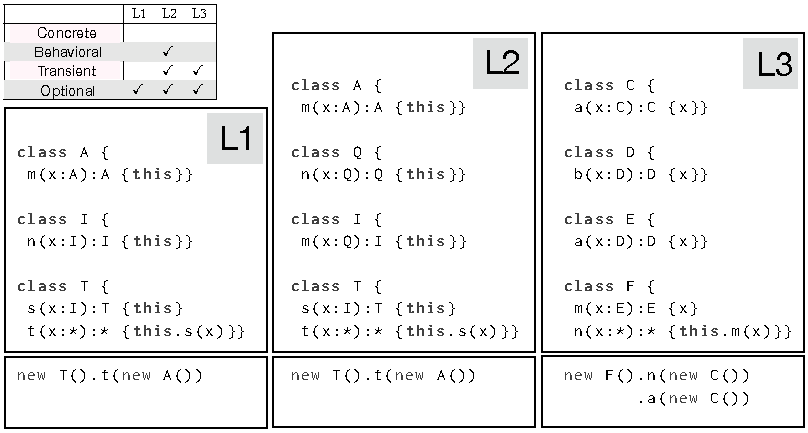
\includegraphics[width=.95\columnwidth]{litm}
\caption{Litmus test. Each program consists of a class table (top) and
an expression (bottom). Top left table indicates successful
executions.}\label{litmus}
\end{figure}

The programs in the litmus test are designed to induce errors. This is done by arranging for
values to cross typed/untyped boundaries in a way that will cause some type
systems to report an error but not others. At heart, these programs can 
be summarized by the
type boundaries that are crossed by an object. The
notation $\C ~\vert_{\,\t}$ denotes an object of class \C passing
through a boundary that expects it to be of type \t. For example,
if method \m expects an argument of type \t, a method call $\e.\m(\ep)$ would
induce the boundary $\ep ~\vert_{\,\t}$. 
In program {\bf L1}, we have:
\[\A ~\vert_{\,\any} ~ \vert_{\,\I}\] 
An instance of 
class \A is first implicitly converted to \any and then to \I; in this program
classes \A and \I are unrelated by subtyping. In {\bf L2}, the same sequence
of conversions is applied:
\[\A~ \vert_{\,\any} ~ \vert_{\,\I}\] 
This time \A and \I both have a
method \m, but the methods have incompatible argument types. Lastly, in
{\bf L3} we start by converting a \C to \any and then to \E
and finally back to \any:
\[\C~ \vert_{\,\any}~\vert_{\,\E}~\vert_{\,\any}\]
The resulting value is then used to call method \m with an argument of class \C.
This correct as method \m in \C does expect an
argument of that type. If the object was an instance of \E instead, the call
would not be legal because \E's method \m expects a class \D as argument.

\subparagraph*{Optional.} An optional gradual type system simply erases all of the
type annotations at run-time; all three programs run to completion without
error.

\subparagraph*{Concrete.} The concrete approach ensures that a
variable of some class \C always refers to an object of that class or of a
subtype of it. To ensure this is the case, all implicit conversions imply a
run-time subtype check. This causes all three programs to fail. {\bf L1}
and {\bf L2} fail on a subtype test \StrSub{}\K\A\I. {\bf L3} fails on the
subtype test \StrSub{}\K\C\E.

\subparagraph*{Behavioral.} The behavioral approach allows
conversion from \any to \C if the value is compatible to \C and if,
after that, it behaves as if it was an instance of \C. The former is
checked by a shallow cast that only looks at method names, and the
latter by a wrapper that monitors further interactions. {\bf L1} fails at
because \A does not have the method \xt n expected by \I. {\bf L2}, however,
executes without error because \A has the method \m expected by \I. {\bf L3} fails, since the instance of \C has been applied
a wrapper for \E. When method \a is called with a \C, the wrapper notices
that \E's method \a expects a \D and that \C and \D are not compatible.

\subparagraph*{Transient.} The transient approach is weaker
than behavioral. It retains the shallow structural checks at casts of the
behavioral approach, but does not wrap values. Transient fails {\bf L1}, for
the same reason as the other two type systems, and passes {\bf L2}, for the
same reason as behavioral. {\bf L3} succeeds because transient forgets that
the \C object was cast to \E.

\subsection{Discussion}

These tests capture the behavior of implementations. The three have been
expressed in TypeScript (optional), StrongScript (concrete), Typed Racket
(behavioral) and Reticulated Python (transient), with the same
errors.\footnote{\url{github.com/BenChung/GradualComparisonArtifact/examples}}
What the litmus tests show is that a precise understanding of the semantics
of gradually typed languages, and their run-time enforcement machinery, is
crucial for developers to know if a program is ``correct.'' Here, all
errors are false positives, since none of these programs performs an invalid
operation. This underlines the fact that in gradually typed language, type
specifications can lead to run-time errors just as faulty code can. Thus,
type annotations must be audited and tested just like code.

These approaches induce usability trade-offs. One way to contextualize this
is with the gradual guarantee of Siek et
al~\cite{GradualGuarantee}. Informally, it states that if there exists a
static type assignment to an untyped program that allows the program to run
to completion, any partial assignment of those types will do too. The
optional approach trivially fulfills this guarantee. Transient likewise
satisfies the gradual guarantee~\cite{Vitousek2017}, as it only checks
top-level structure of values at type boundaries. Unlike optional, transient
does ensure that typed calls succeed; however, a call may produce a dynamic
error if the receiver is of the wrong type (even in a typed context), or the
return is an ill-typed value. The behavioral approach also fulfills the
guarantee, as it only checks arguments and return types when wrappers are
invoked. However, typed function calls can fail if they call an untyped
function that returns the wrong value. Finally, the concrete approach
ensures that every typed call is successful. However, this comes at the
expense of the gradual guarantee -- partially typed classes are not
compatible with more-or-less typed ones. The guarantee
is incompatible with subtyping. Suppose a program were to rely on the
judgment $\{m(\C):\D\} <: \{m(\C):\D\}$. Relaxing the argument type to a
dynamic type, $\{m(\any):\D\} <: \{m(\C):\D\}$, violates subtyping. To
overcome this, Reticulated Python augments subtyping with the aforementioned
consistency relation. This increases the number of programs accepted by the
static type system. However, it is not used by the run-time semantics and
is fundamentally incompatible with the concrete approach (because any use of
consistent subtyping will fail). We omit consistent subtyping.

As an alternative consider the approaches taken by Thorn or
StrongScript. They have three kinds of types: \any (dynamic), \C (concrete),
and \xt{like} \C (optional), combining the concrete and optional approach
into the same language. This design allows for a different kind of
migration; once a program is fully annotated with optional types, they all
can be converted to concrete types without introducing any run-time
errors~\cite{ecoop15}. We do not model this combination directly, as the
underlying details are no different from the concrete approach.

The motivation for making fields private is to simplify the system. With
private fields, errors are limited to method invocation. Field accesses can
be trivially checked; as they are always accessing \this. Moreover, interposing on
method invocation can easily be achieved by wrappers, whereas interposing
on field access would require modifying the code of clients. This would make
the formal development more cumbersome without adding insight.

\section{KafKa: A Core Calculus}\label{kafkacore}

\vspace{-3mm}
\epigraph{\it ``Aux chenilles du monde entier et aux papillons qu’elles
renferment''}

\vspace{-7mm}
\noindent Even without gradual typing, comparing languages is difficult.
Small differences in syntax and features can make even the most similar
languages appear different. As a result, the nuances of gradual type systems
are often hidden amongst irrelevant details. To enable direct comparison,
we propose to translate gradually typed languages down to a common calculus
designed to highlight the distinctions between designs. The target for this
translation is our core language, \kafka. \kafka is a statically typed
language similar to the surface language but with several features added to
enable its use as a common target language.

These additions make an explicit distinction between static and dynamic
operations and replace implicit conversions with explicit casts. \kafka's
first additions consist of two casts which are used at boundaries between
typed and untyped code. The structural subtype cast, written \SubCast\t\e,
ensures that expression \e evaluates to a subtype of \t. The behavioral
cast, written \BehCast\t\e, creates a wrapper around the value of \e that
monitors \e to ensure that it behaves as if it was of type \t.
Additionally, a syntactic distinction is made between static method
invocation, written \KCall\e\m\ep\t\tp, dynamic method invocation,
\DynCall\e\m\ep. Static invocations does not get stuck, whereas
dynamic invocations can. This makes explicit which function calls can fail.

\kafka was designed to align with common statically-typed class-based
object-oriented compilation targets like .NET or the JVM. It maps to the
intermediate language supported by these platforms. \kafka also requires the
ability to generate new classes at run-time, a feature supported by these
environments but typically not present in class-based calculi.

\subsection{Syntax and Semantics}

We had two requirements when designing \kafka: first, to be expressive enough to
capture the dynamic semantics implied by each gradual type system; second,
to have a type system that can express when code is known to be error
free. \kafka's syntax and semantics, loosely inspired by Featherweight
Java~\cite{FJ}, are shown in \figref{fig:kafka}. At the top level, classes
are notated as \Class\C{\fd[1]..}{\md[1]..}; methods, ranged over by \md,
are denoted as \Mdef\m\x\t\t\e; and fields \Fdef\f\t. Expressions consist
of:
\begin{itemize}
\item variables, \x;
\item the self-reference \this; and wrapper target, \that;
\item field accesses, \FRead\f, and field writes, \FWrite\f\e;
\item object creation, \New\C{\e[1]..};
\item static and dynamic method invocations;
\item subtype and behavioral casts;
\item and heap addresses.
\end{itemize}
The static semantics holds only a few surprises; key typing rules appear in
\figref{fig:kafka}. The subtyping relation is inherited from the surface
language. The program typing relation (not shown here), \WFp\e\K, indicates
that expression \e is well-formed with respect to class table \K. The
expression typing judgment $\EnvType \Env\S\K\e\t$, indicates that against
\Env with heap typing \S and class table \K, \e has type \t. Unlike the
surface language, \kafka does not rely on a convertibility relation from
\any to \C and back; instead, explicit casts are required.

Evaluation is mostly standard with an evaluation context consisting of a
class table \K, the expression being evaluated \e, and a heap \s mapping
from addresses \a to objects, denoted $\C\{\a\ldots\}$. Due to the need for
dynamic code generation, the class table is part of the state.

\renewcommand{\S}{\EM{\Sigma}\xspace}

\begin{figure}[!h]\small\noindent\hrulefill

\vspace{4mm}
{\bf Syntax:}
\vspace{2mm}

\begin{tabular}{@{}ll}\hspace{5mm}\begin{minipage}{7.2cm}\begin{tabular}{@{}l@{~}l@{}l@{}l@{}l@{}l@{}l@{}l}
\e\hspace{.1cm} ::= \hspace{.2cm} 
& \x &\B \this &\B \that & \B \\
& \FRead\f &\B \FWrite\f\e &\B \New\C{\e[1]..} &\B\\
& \KCall\e\m\e\t\t &\B \DynCall\e\m\e &\B\\
& \SubCast\t\e &\B \BehCast\t\e & \B \\
& \a &\B \FReadR\a\f &\B \FWriteR\a\f\e 
\end{tabular}\end{minipage}&
\begin{minipage}{2.4cm}\begin{tabular}{l@{~}l@{}l@{}l}
\k &::= ~ \Class \C {\fd[1]..}{\md[1]..} \\
\md &::= ~ \Mdef\m\x\t\t\e \\ 
\fd &::= ~ \Fdef\f\t \\ 
\t &::= ~ \any \B \C \\ 
\K &::= ~ \k \K \B $\cdot$ \\
\S &::= ~ \HT\a\t $\Sigma$ \B $\cdot$ \\
\end{tabular}\end{minipage}\end{tabular}

\vspace{6mm}
{\bf Static semantics:}
\vspace{-2mm}

\begin{mathpar}
\Rule{W6}{
\EnvType \Env\S\K\e\C \\
\Mtype\m\t\tp \in \App\K\C \\
\EnvType \Env\S\K\ep\t
}{
\EnvType \Env\S\K{\KCall\e\m\ep\t\tp}\tp
} 

\Rule{W7}{
\EnvType \Env\S\K\e\any \\
\EnvType \Env\S\K\ep\any
}{
\EnvType \Env\S\K{\DynCall\e\m\ep}\any
} 

\\

\Rule{W9}{
\EnvType \Env\S\K\e\tp
}{
\EnvType \Env\S\K{\SubCast\t\e}\t
}

\Rule{WB}{
\EnvType \Env\S\K\e\tp
}{
\EnvType \Env\S\K{\BehCast\t\e}\t
}

\Rule{W9}{
\S(\a) = \C
}{
\EnvType \Env\S\K\a\C
}

\Rule{W10}{
}{
\EnvType \Env\S\K\a\any
}
\end{mathpar}

\vspace{4mm}
{\bf Execution contexts:}
\vspace{-2mm}

\[
\begin{tabular}{llllllllllllllllll}
\EE &::=& ~ \FWriteR\a\f\EE &\B 
\KCall\EE\m\e\t\t &\B
\KCall\a\m{\EE}\t\t &\B
\DynCall\EE\m\e &\B\\
& & \DynCall\a\m\EE &\B
\SubCast\t\EE &\B
\BehCast\t\EE &\B
\New\C{\a[1]..\,\EE\,\e[1]..} &\B 
\EM{\square}
\end{tabular}
\]

\vspace{4mm}
{\bf Dynamic semantics:}
\vspace{2mm}

\hspace{7mm}\begin{minipage}{\textwidth}

\begin{tabbing}
\K\HS \New\C{\a[1]..} \HS\=\s~\HS\=\Red\HS\=\K\HS\=\ap\HS~\= \sp\HS \= \WHERE\HS\= \fresh\ap \HS\HS\HS\HS\HS\HS\HS\= \sp = {\Map\s{\Bind\ap{\obj\C{\a[1]..}}}}
\\
\K\HS \FReadR\a{\f[i]} \> \s \>\Red\> \K \>$\a[i]$ \> \s \> \WHERE \>\App\s\a=\obj\C{\a[1],\ldots\a[i],\a[n]\ldots}
\\
\K\HS {\FWriteR\a{\f[i]}\ap} \> \s \>\Red\> \K \> \ap \> \sp \> \WHERE \>\App\s\a=\obj\C{\a[1],\ldots\a[i],\a[n]\ldots} \HS 
\\ \> \> \> \> \> \> \> \sp = \Map\s{\Bind\a{\obj\C{\a[1],\ldots\ap,\a[n]\ldots}}}
\\
\K\HS{\KCall\a\m\ap\t\tp} \> \s \>\Red\> \K \> \ep \> \s \> \WHERE\> \ep = {[\a/\this~{\ap/\x}]\e} \HS \\ \> \> \> \> \> \> \> \Mdef\m\x{\t_{1}}{\t_{2}}\e\In \App\K\C \\ \> \> \> \> \> \> \> \App\s\a=\obj\C{\a[1]..} \> \StrSub {\emptyset}\K\t {\t_{1}} \\ 
\> \> \> \> \> \> \> \StrSub {\emptyset}\K{\t_{2}} \tp
\\
\K\HS {\DynCall\a\m\ap}\> \s \>\Red\> \K \> \ep \> \s \> \WHERE\> \ep = {[\a/\this~{\ap/\x}]\e}\HS \\ \> \> \> \> \> \> \> \Mdef\m\x\any\any\e \In \App\K\C \\ \> \> \> \> \> \> \> \App\s\a=\obj\C{\a[1]..} 
\\
\K\HS {\SubCast \any\a} \> \s \>\Red\> \K \> \a \> \s
\\
\K\HS {\SubCast \D\a} \> \s \>\Red\> \K \> \a \> \s \> \WHERE\> \StrSub {\emptyset}\K\C \D \>\App\s\a=\obj\C{\a[1]..} 
\\
\K\HS {\BehCast \t\a} \> \s \>\Red\> \Kp \> \ap \> \sp \> \WHERE\> \behcast \a\t\s\K \Kp\ap\sp 
\\
\K \HS \EM{\EE[\e]} \> \s \>\Red\> \Kp \> \EM{\EE[\ep]} \> \sp \> \WHERE \> \K~\e~\s \Red~\Kp~\ep~\sp
\end{tabbing}
\end{minipage}

\medskip
\hrulefill
\caption{\kafka dynamic semantics and static semantics
(extract).}\label{fig:kafka}
\end{figure}

\subsubsection{Method Invocation}

\kafka has two invocation forms, the dynamic \DynCall\e\m\ep and the static
\KCall\e\m\ep\t\tp, both denoting a call to method \m with argument \ep.
There are several design issues worth discussing. First, as our calculus is
a translation target, it is acceptable to require some explicit preparation
for objects to be used in a dynamic context. A dynamic call is only
successful if the receiver has a method of the expected name and with
argument and return types of \any. This is a design choice of \kafka, even
dynamic invocation has to be well-typed (even if this typing is
trivial). Secondly, it is possible for a static invocation to call an untyped
method (of type \any to \any).
Consider the following
class definition

\begin{tabbing}
\small\hspace{1.5em}\class \C \=\{\\
\>\HS\HS\Mdef\m\x\Int\Int{\HS\x+2\HS}\\
\>\HS\HS\=\m(\x:~\any)~:~\any\{~\SubCast\any{\KCall\this\m{\SubCast\Int\x}\Int\Int}~\}\\
\> \}
\end{tabbing}
assume that class table \K holds a definition for \Int, and that we have
integer constants and addition.
The class demonstrates several features of \kafka. Its class
well-formedness rules (not shown here) allow a limited form of method
overloading. A class may have at most two occurrences of any method \m: one 
``untyped'' with \any as argument and return type; and one,
which we call ``typed'', where either its argument or return type differ from \any.
The static type system enforces a single means of invoking a typed method
\m:
\[\KCall{\New\C{}}\m{2}\Int\Int\] 
Here, the receiver is obviously of type \C and the argument is \Int; thus, the
call is statically well-typed. The expression will therefore 
evaluate the body of \m. For an untyped method, there are two invocation
modes:
\[\DynCall{\New\C{}}\m{2}\]
The call executes correctly here, as \C has an untyped \m. However,
in the general case, there is no guarantee that the receiver of an untyped
invocation has the requested method; and therefore, a dynamic invocation can
get stuck. The receiver of a dynamic invocation has type \any. When the
receiver type is known to be some \C and that class has the requested method,
then the static invocation can be used:
\[\KCall{\New\C{}}\m{2}\any\any\]
The invocation will succeed. All nuances of invocation
will come in handy when translating the surface language to \kafka.

\subsubsection{Run-time Casts}

\kafka has two cast operations: the structural subtype cast $\SubCast\t\e$ and the
behavioral cast $\BehCast\t\e$, both indicating the desire for the result
of evaluating \e to be of type \t. Where the casts differ is what is meant by
``has type \t''. The subtype cast checks that the result of evaluating \e
is an object whose class is compatible with \t. If \t is a class, then it
will check for a subtyping relation; otherwise, if \EM{\t=\any}, the cast 
will succeeds. As every value in the heap is
tagged by its type constructor, it is always possible to perform this check. 
The behavioral cast is more complex; we will
describe it in the remainder of this section.

The objective of the behavioral cast is to ensure that the wrapped object
behaves as the target type dictates. When given the address \a of some
object, this cast creates a wrapper object, say \ap, that enforces the 
invariant that \a \emph{behaves} as a
value of type \t. Function \behcastE\a\t\s\K \Kp\ap\sp specifies its
semantics, shown in \figref{behavetext}. There are two cases to consider:
either the target type is a class \Cp, or it is \any.

\begin{figure}[t]\hrulefill\small

\vspace{4mm}
{\bf Behavioral cast:}
\vspace{4mm}
\behcastE\a\t\s\K \Kp\ap\sp\\[2mm]
\begin{tabular}{ll|ll}
\a & Reference to wrap & \ap & Wrapped reference \\
\t & Target type to enforce & \Kp & Class table with wrapper\\ 
\s & Original heap & \sp & New heap \\
\K & Original class table &
\end{tabular}

\vspace{4mm}

\begin{equation*}
\behcastE\a\Cp\s\K \Kp\ap\sp \HS\WHERE\HS \begin{cases}
\HS\App\s\a = \obj\C{\a[1]..} \HS\HS \fresh{\D,\ap} \HS\HS
\sp = \Map \s{\Bind\ap{\obj\D{\a}}} \\\HS
\md[1].. \In\App\K\C \HS\HS \names{\mdp[1]..} \subseteq \names{\md[1]..} \\\HS
\mdp[1].. \In \App\K\Cp \HS\HS \cload{\md[1]..} \HS \cload{\mdp[1]..} \\\HS
\Kp = \K ~\wrap\C{\md[1]..}{\mdp[1]..}\D 
\end{cases}
\end{equation*}

~\\[-8mm]

\begin{equation*}
\behcastE\a\any\s\K \Kp\ap\sp \HS\HS\WHERE\HS\HS\begin{cases}\HS
\App\s\a = \obj\C{\a[1]..} \HS\HS \md[1].. \In \App\K\C \HS\HS
\fresh{\D,\ap} \\\HS \cload{\md[1]..} \HS\HS
\Kp = \K ~ \wrapAny\C{\md[1]..}\D \\\HS
\sp = \Map \s{\Bind\ap{\obj\D{\a}}} 
\end{cases}\end{equation*}

\vspace{4mm}

\hspace{8mm}\begin{minipage}{12cm}\begin{tabbing}\small
\wrap\C{\md[1]..}{\mdp[1]..}\D = \src{\Class\D{\Fdef\that\C}{\mdpp[1]..}}\\
\HS\HS\WHERE\HS\= \Mdef\m\x{\t[1]}{\t[2]}\e\In\md[1].. \\
\> \mdpp[1] =\= \src{\Mdef\m\x{\tp[1]}{\tp[2]}{~\BehCast{\tp[2]}{\KCall{\FRead\that}\m{\bscast{\tp[1]}\x}{\t[1]}{\t[2]}}}} .. \\
\> \> \HS\HS \= \textbf{if} \HS \Mdef\m\x{\tp[1]}{\tp[2]}\ep\In\mdp[1].. \\
\\[-3mm]
\> \> \src{\Mdef\m\x{\t[1]}{\t[2]}{~\KCall{\FRead\that}\m{\x}{\t[1]}{\t[2]}}} .. \\ \> \> \HS\HS \textbf{otherwise}
\\[2mm]
\wrapAny{\C}{\md[1]..}{\D} = \src{\Class \D{ \Fdef\that\C}{ \mdp[1]..}}\\
\HS\HS\WHERE\HS\=\mdp[1] = \src{ \Mdef\m\x{\any}{\any}{~\BehCast\any{ \KCall{\FRead\that} \m {\bscast{\t}\x}{\t}{\tp}} } } ..
\HS\HS\HS\HS \\ \> \> \HS\HS \= \textbf{if} \HS \Mdef\m\x{\t}{\tp}\e\In\md[1].. \\
\end{tabbing}\end{minipage}

\vspace{-2mm}

\hrulefill
\caption{Behavioral cast semantics.}\label{behavetext}
\end{figure}

If the target type is \Cp, then \behcastS\a\Cp\s\K will return an updated
class table \Kp, a reference to the wrapped object \ap, and an updated heap
\sp. As long as \a has every method name specified by \Cp, the cast itself
will succeed. If \a is missing a method, it is impossible for \a to
implement \Cp correctly, and early failure is indicated. Otherwise, the
metafunction continues to generate a type wrapper. Class generation itself
is delegated to the \W metafunction. A \W invocation,
\EM{\W(\C,\md_1..,\mdp_1.., \D)}, takes a class \C, a fresh name \D, and two
method lists $\md_1..$ and $\mdp_1$, respectively the method of \C and the
methods of the type to enforce. The class generated by \W will have adapter
methods for each method \m occurring in both $\md_1..$ and $\mdp_1..$. Type
mismatches between the wrapped object and the wrapping type are resolved
with more behavioral casts. For methods that do not need to be adapted
(methods only in $\md_1..$), a simple pass-through method is generated. This
method simply calls the wrapped object; itself referred to by the
distinguished variable \that.

If the target type is \any, the wrapper class is simpler. It only needs to
check that method arguments match the types expected by the wrapped
object. This is done by another behavioral cast. Return values are cast to
\any.

For example, consider the following program which has two classes \C and \D.
Even though \C and \D both have method \a, they are not subtypes because the
arguments to their \m implementations are not related.

\begin{tabbing}\small
\hspace{1.5em}
\Call{(\BehCast\C{(\BehCast\D{\New\C{}})})}{\xt{b}}{2} \HS\HS\HS\WHERE\HS
\K\HS =\HS \= \class\= \C \{\\
\> \HS \Mdef\m\x\any\any{\HS\x\HS}\\
\> \HS \Mdef\n\x\any\any{\HS\x\HS}\\
\> \} \\
\>\class \D \{\HS \Mdef\m\x\Int\Int{\HS\x\HS}\HS \}
\end{tabbing}
The program starts with a \C, casts it to \D, and then back to \C. The
reason we generate pass-through methods (the wrapper that enforces type \D
has a method \n) is that without them, the method \n would be ``lost''. 
Without the pass-through method, it would be impossible to cast back to
\C, as the wrapper would only have an implementation for \m. Wrappers
with this semantics are referred to as opaque, as it is not possible
to see methods of the underlying object though them. In contrast,
\kafka uses transparent wrappers.
To illustrate what this looks like, the following class \xt E is generated
by the cast from \C to \D:

\begin{tabbing}\small
\hspace{1.5em}
\HS\HS\=\class\= \xt E \{\\
\>\> \HS \Fdef\that\C \\
\>\> \HS \Mdef\m\x\Int\Int{\HS\BehCast\Int{\KCall\that\m{\BehCast\any\x}\any\any\HS}} \\ 
\>\> \HS \Mdef\n\x\any\any{\HS \KCall\that\n{\x}\any\any\HS} \\ 
\>\}
\end{tabbing}
By keeping \n present, it is possible to return an instance of
\E to \C again. If we were to remove \n, then \xt E would no longer
be convertible back to \C again. 

\subsection{Type soundness}

The \kafka type soundness theorem ensures that a well-formed program can
only get stuck at a dynamic invocation, a subtype cast, or a behavioral
cast, and only there when justified.

\begin{theorem}[\kafka type soundness]
For every well-formed state $\WFq{\K~\e~\s}$ and well-typed
expression $\EnvType\emptyset\S\K\e\t$, where heap typing \S is obtained by
mapping the class of each object to the corresponding address, one of the
following holds:
\newcommand{\Sp}{\EM{\S'}\xspace}
\begin{itemize}
\item There exists some reference \a such that $\e = \a$.
\item $\K~\e~\s\Red\Kp~\ep~\sp$, where $\WFq{\Kp~\ep~\sp}$,
\EnvType\emptyset\Sp\Kp\ep\t, \sp has all of the values of \s, \Sp has all of the
types of \sp, and \Kp has all of the classes of \K.
\item $\e=E[\DynCall\a\m\ap]$ and \a refers to an object without a method \m.
\item $\e=E[\SubCast\C\a]$, and \a refers to an object whose class is not
a subtype of \C.
\item $\e=E[\BehCast\C\a]$, and \C contains a method that \a does not.
\end{itemize}
\end{theorem}
The proof is mostly straightforward, with one unusual case, centered around
the \xt{bcast} metafunction. When the \xt{bcast} metafunction is used to
generate a wrapper class, which is then instantiated, producing a new class
table and heap, we must then show that the new class table is well formed,
that the new heap is also well formed, and that the new wrapper is a subtype
of the given type \C. Proving these properties is relatively easy. Class
table well-formedness follows by construction of the wrapper class and by
well-formedness of the old class table. Heap well-formedness follows by
well-formedness of the class table, construction of the new heap, and
well-formedness of the old heap. Proving that the type of the wrapper is a
subtype of the required type proceeds by structural induction over the
required type. The proof of soundness has been formalized in Coq and is
available in the supplementary material. The proof relies on two axioms
dealing with recursive structural subtyping. We did not prove these as
they have been shown in prior work~\cite{JonesStructural}.

\subsection{Discussion}

The design of \kafka's two invocation forms bears discussion. In some
previous works, dynamic invocation has been implemented by a combination of
a cast and a statically typed call. In our case, following this approach
would require creating a type for each invocation (as was done
in~\cite{popl10}). Instead, providing a dynamic invocation form seemed more
natural. The use of explicitly typed invocation is a result of our desire
to be able to rule out more errors statically. Whenever a translation can
generate a static invocation, the soundness result ensure that the call will
succeed. But, some methods need to be called from both a typed and untyped
context, to achieve this we generate two versions of the method and leverage
the difference between typed and untyped calls to express invovations
occuring in each context.

One of our requirements for \kafka was that it support transparent wrappers
as these are needed for the behavioral approach. The combination of
structural subtyping and dynamic class generation allows to generate
subtypes on the fly. These subtypes have all the methods of the target type
plus some new ones. The choice of having fields be private means that the
wrappers do not have to special case field access. If fields were accessible
from outside the object, some more complex rewritting would have to be
used.

\kafka was intended to match the intermediate languages of commercial VMs.
To validate this, we implemented a compiler from \kafka to
C\#.\footnote{\small\url{github.com/BenChung/GradualComparisonArtifact/netImpl}}
The only challenge was due to subtyping. \kafka uses structural typing,
while C\# is nominal, and \kafka allows methods in subtypes to be
contra-variant in argument and co-variant in return type, while C\# requires
invariance. Implementing structural subtyping on top of a nominally typed
language is tricky. Structural types create implicit subtyping
relationships, which the nominal type system expects to be explicit. Prior
work used reflection and complex run-time code
generation~\cite{StructuralTypesOnJVM}, but this is needlessly complex for a
proof of concept. Instead, we reify the implicit relationships introduced
by structural subtyping into explicit nominal relationships by generating
interfaces. Given two classes \C and \D, where $\K\vdash \C \Sub \D$ holds,
we generate two interfaces \xt{CI} and \xt{DI}, where \xt{CI} is declared to
extend \xt{DI}. As a result, if two types are subtypes, their corresponding
C\# interfaces will be as well. The next problem is that \kafka allows
subtype methods to be contra-variant in argument and co-variant in return
types. As a result, a single method in \xt{CI} may not be sufficient to
implement \xt{DI}. We solve this by having every class's C\# equivalent
implement every interface explicitly, with each explicit implementation
delegating to the real, most general, implementation. Despite these issues,
we were able to accurately translate \kafka types. We translate static and
dynamic invocations into corresponding C\# invocations since C\# also has a
dynamic type. The underlying run time can then use the translated \kafka
types to perform method dispatch, while inserting dynamic checks wherever
the \kafka code calls for an untyped invocation. This prototype shows that
\kafka primitives are close to those of intermediate languages. As a result,
the translation of gradual type systems to \kafka provides insight as to how
they might be implemented.


\section{Translating Gradual Type Systems}

\vspace{-4mm}

\epigraph{\small\it ``Was ist mit mir geschehen? dachte er.
Es war kein Traum''}

\vspace{-7mm}

\noindent Equipped with the source and target languages, we can describe
the gradual-to-statically typed translation from source to \kafka.
Each semantics is translated through a function mapping well-typed
surface programs into well-typed \kafka terms. The translation
explicitly determines which type casts need to be inserted and the
invocation forms to use. A type-driven translation will insert casts
where the surface language used consistency.

\subsection{Class Translation}

The translations for surface level classes are shown in
\figref{fig:traclass}. Each class in the surface language translates to a
homonymous \kafka class, retaining type names through translation.
The grey background denotes code generated in the translation.
The notation \EM{\e;\ep} denotes sequencing. 

\begin{figure}[t] {\small \hrulefill\\
\begin{tabular}{llc@{\hspace{.25cm}}l} \\[-2mm]

{\bf Optional:} \\[1mm]

\HS\TR[\OTS]{\Class\C{\fd[1]..}{\md[1].. }}
& = \src{\Class\C{\fdp[1]..}{\mdp[1]..}}\\ 
& \WHERE\HS\HS\HS \fdp[1] = \src{\Ftype\f\any}..\HS\HS \fd[1] = \Ftype\f\t..\\
& \HS\HS\HS\HS\HS\HS\HS\HS\HS \mdp[1] = \src{\Mdef\m\x\any\any\ep}..\\ 
& \HS\HS\HS\HS\HS\HS\HS\HS\HS \md[1] = \Mdef\m\x{\t[1]}{\t[2]}\e \HS\HS
\ep=\;\TR[\OTS]{\e}\\ 

{\bf Transient:} \\[1mm] 
\HS\TR[\TTS]{\Class\C{\fd[1]..}{\md[1]..}}
& = \src{\Class\C{\fdp[1]..}{\mdp[1]..}}\\ 
& \WHERE \HS\HS\HS \fdp[1] = \src{\Ftype\f\any} .. \HS 
\fd[1] = \Ftype\f\t ..\HS\HS \\ 
& \HS\HS\HS\HS\HS\HS\HS\HS\HS \mdp[1] = \src{\Mdef\m\x\any\any{\SubCast\t\x ~; ~\ep[1]}} .. \\ 
& \HS\HS\HS\HS\HS\HS\HS\HS\HS \md[1] = \Mdef\m\x\t\tp\e .. 
\HS \HS \ep[1] = \TAG[\TTS]\e{\x:\t\,\this:\C}\any~ .. \\ 

{\bf Behavioral:} \\[1mm]
\HS\TR[\BTS]{\Class\C{\fd[1]..}{\md[1].. }} 
& = \src{\Class \C {\fd[1]..}{\mdp[1].. } } \\ 
& \WHERE \HS\HS\HS \mdp[1] = \src{\Mdef\m\x\t\tp{\ep[1]}} ..\HS\HS \\ 
& \HS\HS\HS\HS\HS\HS\HS\HS\HS \md[1] = \Mdef\m\x\t\tp{\e[1]} ..\HS\HS 
\HS\HS \ep[1] = \TRG[\BTS]{\e[1]}{\x:\t\,\this:\C} \\ 

{\bf Concrete:} \\[1mm]

\HS\TR[\CTS]{\Class\C{\fd[1]..}{\md[1].. }} 
& = \src{ \Class \C{ \fd[1]..}{\mdp[1].. \mdpp[1]..}} \\ 
& \WHERE \HS\HS\HS {\mdp[1]} = \src{\Mdef\m\x{{\t[1]}}{{\t[2]}}{\ep}} .. \\ 
& \HS\HS\HS\HS\HS\HS\HS\HS\HS \md[1] = \Mdef\m\x{\t[1]}{\t[2]}\e .. 
\HS\HS \ep = \TAG[\CTS]{\e}{\this:\C\,\x:\t[1]}{\t[2]}~ ..\\
& \HS\HS\HS\HS\HS\HS\HS\HS\HS {\mdpp[1]} = \src{\Mdef\m\x\any\any{\SubCast\any{\KCall\this\m{\SubCast{{\t[1]}}\x}{\t[1]}{\t[2]}}}} \\ 
& \HS\HS\HS\HS\HS\HS\HS\HS\HS\HS \HS\HS\HS\HS\HS\HS\HS\HS\HS\HS\HS \textbf{\IF} {\t[1]} $\neq$ \any \\ 
& \HS\HS\HS\HS\HS\HS\HS\HS\HS \HS\HS\HS\HS\HS\HS \src{empty} 
\HS {\bf otherwise} .. 
\end{tabular} \\[-2mm]

\hrulefill}
\caption{Translations for classes.} \label{fig:traclass} 
\end{figure}

\subparagraph*{Optional.} The optional approach provides no
correctness guarantees. Retaining the surface type annotations through
translation would not preserve this semantics, so we erase them. The
resulting class has all fields, all method arguments, and all return
values typed as \any.

\subparagraph*{Transient.} In the transient approach, ensure
that for any method call, the receiver does have a method with the
corresponding name. To encode this within the \kafka type system requires
replacing all of the argument and return types with \any. This translation
allows functions to be called under any type and to return values of any
type. Casts to the erased types are then effectively shallow structural
checks only. As there is no
guarantee that fields contain values of their type,
the translation sets their type to \any.

\subparagraph*{Behavioral.} The behavioral approach guarantees
soundness by wrapping values that cross type-untyped boundaries. Methods
are preserved by the translation but bodies are translated.

\subparagraph*{Concrete.} The concrete approach ensures that
variables of non-\any types refer to subtypes of the given type. Each method
appearing in the original class is retained as such with its body
translated. Moreover, all typed methods could be called from an untyped
context, so untyped variants are generated that guard the typed functions.
These variants perform subtype casts on their arguments to ensure that they
were given the right types, then call the guarded typed function.

\subsection{Expression Translation} 

To accommodate differences between the gradual typing semantics, we use two
different expression translation schemes. The first is a type-agnostic
one, used for the optional approach. $\TR[\OTS]\e$ denotes optional translation,
where \e is the target expression, and the result is a \kafka term. We use
this form to simplify the optional translation, as it is ambivalent about the
types of the expressions it is translating; the optional semantics simply
eliminates all of them.

\enlargethispage{2\baselineskip}
The second translation form is type-aware, used for the three other
approaches. The type-aware translation has two forms, $\TRG[\SOMS]\e\Env$
and $\TAG[\SOMS]\e\Env\t$, inspired by work on bidirectional
type-checking~\cite{pierce:1998:local}. The first form,
$\TRG[\SOMS]\e\Env$, is analogous to the synthetic case in bidirectional
type-checking. It is used for expressions without any specific required
type. The second form, $\TAG[\SOMS]\e\Env\t$, is used when \e must have
some type \t. Analogous to the analytic case of bidirectional type-checking,
this form applies when some enclosing expression has an expectation of the
type of \e. For example, it is used in translation of method arguments,
which must conform to the types of the arguments to the method. We refer to
this as assertive translation. These two forms allow us to identify where
consistency was needed to conclude the surface level typing judgment.

\begin{figure}[h]\small \hrulefill\\[2mm]
\begin{tabular}{llc@{\hspace{.25cm}}l@{\HS}l@{\HS}l}

{\bf Transient:}\\[1mm]
\HS \TAG[\TTS]\e\Env\t & = \src\ep &\WHERE
& \TypeCk{\K,\Env}\e\tp
& \EM{\K\vdash\tp\Sub\t}
& \ep = \TRG[\TTS]\e\Env \\
\HS\TAG[\TTS]\e\Env\t &= \src{\SubCast\t\ep} &\WHERE
& \TypeCk{\K,\Env}\e\tp 
& \EM{\K\vdash \tp \not \Sub \t}
& \EM{\ep = \TRG[\TTS]\e\Env} \\[2mm]
{\bf Behavioral:} \\ [1mm]
\HS\TAG[\BTS]\e\Env\t & = \src\ep & \WHERE
& \TypeCk{\K,\Env}\e\tp
& \EM{\K\vdash \tp \Sub \t}
& \ep = \TRG[\BTS]\e\Env\\
\HS\TAG[\BTS]\e\Env\t & = \src{\BehCast\t\ep} & \WHERE
& \TypeCk{\K,\Env}\e\tp \HS 
& \EM{\K\vdash \tp \not \Sub \t}
& \ep = \TRG[\BTS]\e\Env \\[2mm]
{\bf Concrete:} \\[1mm]
\HS\TAG[\CTS]\e\Env\t &= \src\ep &\WHERE
& \TypeCk{\K,\Env}\e\tp 
& \EM{\K\vdash\tp \Sub \t} 
& \ep = \TRG[\CTS]\e\Env\\
\HS\TAG[\CTS]\e\Env\t &= \src{\SubCast{\t}\ep} &\WHERE
& \TypeCk{\K,\Env}\e\tp 
& \EM{\K\vdash\tp \not\Sub \t}
& \EM{\ep = \TRG[\CTS]\e\Env} 
\end{tabular}
\\

\hrulefill

\caption{Assertive translation.}\label{fig:trtype}
\end{figure}

The assertive translation of \figref{fig:trtype} is responsible for producing
well-typed terms by adding casts into expressions where static types differ.
The rules closely track the convertibility relation of the surface language.
Every type-driven translation has two cases. The first case is used when the
required type happens to be a supertype of the expression's actual type, in
which cast upcasting can happen implicitly and no further action is required.
The second case handles typed-untyped boundaries, conversions to or from \any.
The concrete and transient approaches both use the subtype cast operator to
protect these boundaries, though the effective semantics are different; concrete
retains the types that transient erases, so subtype casts in transient check
structural compatibility (e.g. are all the needed methods present) alone
whereas concrete subtype casts check the entire object's types.
The behavioral approach instead inserts behavioral casts
at boundaries.

\enlargethispage{1.5\baselineskip}
The translation of field access appears in \figref{fig:travar}. The
optional translation only inserts a cast to \any in front of uses 
\this as a technicality required for statically typing terms. The
transient translation casts variables and fields to their statically
expected type, as their values may be of any type. In transient, however,
subtype casts only check the structure of the types. The behavioral
translation and the concrete translation leave both types of access intact.

\begin{figure}[h!]\small\hrulefill\\
\begin{tabular}{@{}l@{\HS}l}
\\[-2mm]

\begin{tabular}{llc@{\hspace{.25cm}}l@{\HS}l@{\HS}l}

{ \bf Optional:} \\[2mm]
\HS\TR[\OTS]\x & = \src \x \\
\HS\TR[\OTS]\this & = \src{\SubCast\any\this} \\
\HS\TR[\OTS]{\FRead\f} & = \src{\FRead\f} \\
\\
\end{tabular}
&
\begin{tabular}{llc@{\hspace{.25cm}}l@{\HS}l@{\HS}l}
{ \bf Transient:}\\[2mm]
\HS\TRG[\TTS]\x\Env & = \src{\SubCast\t\x} & \WHERE & \TypeCk{\K,\Env}\x\t \\
\HS\TRG[\TTS]\this\Env & = \src\this \\
\HS\TRG[\TTS]{\FRead\f}\Env & = \src{\SubCast\t{\FRead\f}} & \WHERE & \TypeCk{\K,\Env}\this\C \HS \Ftype\f\t\In\App\K\C \\
\end{tabular}
\\
\begin{tabular}{llc@{\hspace{.25cm}}l@{\HS}l@{\HS}l}		
{ \bf Behavioral:} \\[2mm]
\HS\TRG[\BTS]\x\Env &= \src{\x} \\
\HS\TRG[\BTS]\this\Env &= \src{\this} \\
\HS\TRG[\BTS]{\FRead\f}\Env &= \src{\FRead\f}
\end{tabular}
&
\begin{tabular}{llc@{\hspace{.25cm}}l@{\HS}l@{\HS}l}		
{\bf Concrete:}\\[2mm]
\HS\TRG[\CTS]{\x}\Env & = \src \x \\
\HS\TRG[\CTS]\this\Env &= \src{\this} \\
\HS\TRG[\CTS]{\FRead\f}\Env & = \src{\FRead\f}
\HS\end{tabular}
\end{tabular}\\

\hrulefill
\caption{Translations variables and field access.}\label{fig:travar}
\end{figure}

The translation for assignment is shown in \figref{fig:trassn}. All the
approaches translate the value only differing in the expected
type. Behavioral and concrete require that the result has the statically
known type, transient expects \any, and the optional semantics imposes no
type requirement whatsoever.
\enlargethispage{-1\baselineskip}

\begin{figure}[h!]\small
\hrulefill\\
\begin{tabular}{llc@{\hspace{.25cm}}l@{\HS}l@{\HS}l}\\[-1mm]

{\bf Optional:}\\[1mm]
\HS\TR[\OTS]{\FWrite\f\e} 
& = \src{\FWrite\f\ep} &\WHERE&\ep=\TR[\OTS]\e\\[2mm]
{\bf Transient:}\\[1mm]
\HS\TRG[\TTS]{\FWrite\f\e}\Env & = \src{{\FWrite\f\ep}} &\WHERE
& \TypeCk{\K,\Env}\this\C
& \Ftype\f\t\In\App\K\C 
& \ep = \TAG[\TTS]\e\Env\any\\[2mm]
{\bf Behavioral:}\\ [1mm]
\HS\TRG[\BTS]{\FWrite\f\e}\Env &= \src{\FWrite\f\ep} & \WHERE
& \TypeCk{\K,\Env}{\this}\C
& \Ftype\f\t\In\App\K\C 
& \ep = \TAG[\BTS]\e\Env\t\\[2mm]
{\bf Concrete:}\\[1mm]
\HS\TRG[\CTS]{\FWrite\f\e}\Env & = \src{\FWrite\f\ep} & \WHERE
& \TypeCk{\K, \Env}\this\C
& \Ftype\f\t\In\App\K\C
& \ep = \TAG[\CTS]\e\Env{\t} 
\end{tabular}\\[-2mm]

\hrulefill\vspace{1mm}
\caption{Translations for assignment.}\label{fig:trassn}
\end{figure}
\begin{figure}[h!]\small
\hrulefill\\
\begin{tabular}{llc@{\hspace{.25cm}}l@{\HS}l@{\HS}l}
\\[-2mm]
{\bf Optional:}\\[1mm]
\HS\TR[\OTS]{\New\C{\e[1]..}} & = \src{\SubCast\any{\New\C{\ep[1]..}}} &\WHERE 
& \ep[1] = \TR[\OTS]{\e[1]} .. \\[2mm]
{\bf Transient:}\\[1mm]
\HS\TRG[\TTS]{\New\C{\e[1]..}}\Env &= \src{\New\C{\ep[1]..}} &\WHERE 
& \Ftype{\f[1]}{\t[1]}\In\App\K\C
& \ep[1] = \TAG[\TTS]{\e[1]}\Env{\any} ~.. \\[2mm]
{\bf Behavioral:}\\ [1mm]
\HS\TRG[\BTS]{\New\C{\e[1]..}}\Env & = \src{\New\C{\ep[1]..}} &\WHERE 
& \Ftype{\f[1]}{\t[1]}\In\App\K\C
& \ep[1] = \TAG[\BTS]{\e[1]}\Env{\t[1]} ~..\\
{\bf Concrete:} \\[1mm]
\HS\TRG[\CTS]{\New\C{\e[1]..}}\Env &= \src{\New\C{\ep[1]..}} &\WHERE
& \Ftype{\f[1]}{\t[1]}\In\App\K\C
& \ep[1] = \TAG[\CTS]{\e[1]}\Env{\t[1]} ..
\end{tabular}\\[-2mm]

\hrulefill\vspace{1mm}
\caption{Translations for object creation.}\label{fig:tranew}
\end{figure}
\begin{figure}[h!]\small
\hrulefill\\
\\[-2mm]
\begin{tabular}{llc@{\hspace{.25cm}}l@{\HS}l@{\HS}l}
{\bf Optional:}\\[1mm]
\HS\TR[\OTS]{\Call{\e[1]}\m{\e[2]}} &= \src{\DynCall{\ep[1]}\m{\ep[2]}} &\WHERE 
& \ep[1] = \TR[\OTS]{\e[1]} & \ep[2] = \TR[\OTS]{\e[2]} \\[2mm]
{\bf Transient:} \\[1mm]
\HS\TRG[\TTS]{\Call{\e[1]}\m{\e[2]}}\Env 
& = \src{\DynCall{\ep[1]}\m{\ep[2]}} & \WHERE 
& \TypeCk{\K,\Env}{\e[1]}\any 
& \ep[1] = \TRG[\TTS]{\e[1]}\Env
& \ep[2] = \TAG[\TTS]{\e[2]}\Env\any \\ 
\HS\TRG[\TTS]{\Call{\e[1]}\m{\e[2]}}\Env 
& = \src{\SubCast{\D[2]}{\KCall{\ep[1]}\m{\ep[2]}\any\any}}
& \WHERE
& \TypeCk{\K,\Env}{\e[1]}\C 
& \ep[1] = \TRG[\TTS]{\e[1]}\Env 
& \ep[2] = \TAG[\TTS]{\e[2]}\Env{\any} \\
& & & \multicolumn{2}{l}{\Mtype\m{\D[1]}{\D[2]}\In\App\K\C} \\[2mm]
{\bf Behavioral:}\\[1mm]
\HS\TRG[\BTS]{\Call{\e[1]}\m{\e[2]}}\Env 
& = \src{\DynCall{\ep[1]}\m{\ep[2]}} & \WHERE
& \TypeCk{\K,\Env}{\e[1]}\any
& \ep[1] = \TRG[\BTS]{\e[1]}\Env
& \ep[2] = \TAG[\BTS]{\e[2]}\Env\any
\\
\HS\TRG[\BTS]{\Call{\e[1]}\m{\e[2]}}\Env & = \src{\KCall{\ep[1]}\m{\ep[2]}{\D[1]}{\D[2]}} & \WHERE 
& \TypeCk{\K,\Env}{\e[1]}\C 
& \ep[1] = \TRG[\BTS]{\e[1]}\Env
& \ep[2] = \TAG[\BTS]{\e[2]}\Env{\D[1]} \\
& & & \multicolumn{2}{l}{\Mtype\m{\D[1]}{\D[2]}\In\App\K\C} \\[2mm]
{\bf Concrete:}\\[1mm]
\HS\TRG[\CTS]{\Call{\e[1]}\m{\e[2]}}\Env 
& = \src{\DynCall{\ep[1]}{\m}{\ep[2]}} & \WHERE 
& \TypeCk{\K,\Env}{\e[1]}\any 
& \ep[1]= \TRG[\CTS]{\e[1]}\Env 
& \ep[2] = \TAG[\CTS]{\e[2]}\Env\any\\
\HS\TRG[\CTS]{\Call{\e[1]}\m{\e[2]}}\Env 
& = \src{\KCall{\ep[1]}{\m}{\ep[2]}{\D[1]}{\D[2]}} 
& \WHERE & \TypeCk{\K,\Env}{\e[1]}\C 
& \ep[1] = \TRG[\CTS]{\e[1]}\Env 
& \ep[2] = \TAG[\CTS]{\e[2]}\Env{\D[1]} \\ 
& & & \multicolumn{2}{l}{\Mtype\m{\D[1]}{\D[2]}\In\App\K\C} & \\
\end{tabular}\\
\hrule	\vspace{1mm}
\caption{Translations for function invocation.}\label{fig:trafuninv}
\end{figure}

\enlargethispage{-1.0\baselineskip}

The translation for object creation, shown in \figref{fig:tranew}, follows
the same reasoning. It inserts casts for each argument to be the required type
according to class translation.

The translations for invocation are shown in \figref{fig:trafuninv}. The
optional approach translates all invocations to dynamic invocation, as it
cannot provide any static guarantee. In the concrete and behavioral
approaches, since the static types are retained, arguments must be asserted
to have the statically known type. In the transient semantics, the argument
type is ignored, so the argument to a statically typed method call is only
required to be of type \any, but the return type is checked. In all of the
systems, if the type of the receiver is \any, dynamic invocation is used.

\pagebreak
\subsection{Example}

We illustrate the translation with the behavior of litmus program {\bf L3}.
The operational principle of {\bf L3} is that it creates a new object (an
instance of \C), then uses an untyped intermediate to represent it as type
\E. Type \E ascribes the wrong type for argument \x, substituting \D for the
correct type \C. 

\begin{figure}[h!]\small
\hrulefill\\
\\
\begin{tabular}{l}
{\bf Source:} \\[2mm]
\(
\begin{array}{l@{\,}l}
\Class{\xt F}{}{&\Mdef\m\x{\xt E}{\xt E}\x \HS\HS
\Mdef\n\x\any\any{\Call\this\m\x}} \\
\end{array}
\) \\[2mm]
{\bf Optional:}\\[2mm]
\(
\begin{array}{l@{\,}l}
\Class{\xt F}{}{&\Mdef\m\x{\any}{\any}\x \HS\HS
\Mdef\n\x\any\any{\DynCall{(\SubCast\any\this)}\m\x}} 
\end{array}
\) \\[2mm]
{\bf Transient:}\\[2mm]
\(
\begin{array}{l@{\,}l}
\Class{\xt F}{}{
&\Mdef\m\x\any\any{\SubCast{\xt E}{\x}; ~ \SubCast{\any}{\x} } 
\HS\HS \Mdef\n\x\any\any{\SubCast{\any}{\x}\sspce 
\SubCast{\any}{\SubCast{\xt E}{\KCall\this\m{\SubCast\any{\SubCast\any\x}}\any\any}}}} 
\end{array}
\)\\[2mm]
{\bf Behavioral:} \\[2mm]
\(
\begin{array}{l@{\,}l}
\Class{\xt F}{}{&\Mdef\m\x{\xt E}{\xt E}\x \HS\HS
\Mdef\n\x\any\any{\BehCast\any{\KCall\this\m{\BehCast{\xt E}\x}{\xt E}{\xt E}}}} 
\end{array}
\) \\[2mm]
{\bf Concrete:} \\[2mm]
\(
\begin{array}{l@{\,}l}
\Class{\xt F}{}{&\Mdef\m\x{\xt E}{\xt E}\x \HS\HS
\Mdef\n\x\any\any{\SubCast\any{\KCall\this\m{\SubCast{\xt E}\x}{\xt E}{\xt E}}}} 
\end{array}
\) \\
\end{tabular}\vspace{2mm}\\
\hrule\vspace{4mm}

\caption{Class translation for litmus test L3.} \label{fig:l3trans}
\end{figure}

\enlargethispage{-1\baselineskip}
Two of the gradual type systems notice this invalid type. Concrete errors on
{\bf L3} because \E is not a subtype of \C. With behavioral, the unused
type ascription is saved as a wrapper and is enforced causing a run-time error.

While this reasoning provides an intuition, it provides few detail for which
we turn to our formalism. We present the translation from the top, starting
with classes in \figref{fig:l3trans}. The optional approach does no
checking whatsoever, and simply erases types. Transient also erases types,
but adds argument casts on method entry. In the case of \m, argument \x is
checked to be of type \E, as the translation of type \E does not include
types no type error will be reported. Behavioral retains typed methods but
adds behavioral casts on untyped methods. The concrete semantics retains
typed methods, and adds a subtype cast when a variable of type \any is passed
to a method that expects and \E.

\begin{figure}[h!]\small
\hrulefill\\
\\
\begin{tabular}{rl}
\multicolumn{2}{l}{\begin{tabular}{l}
{\bf Source:}\\[2mm]
\(\begin{array}{l@{\,}l} 
\Class{\xt E}{}{&\Mdef\m\x{\xt D}{\xt D}\x } \\
\end{array}\) 
\end{tabular}}
\\[2mm]\\
\begin{tabular}{@{}l}
{\bf Optional:}\\[2mm]
\(\begin{array}{l@{\,}l}
\Class{\xt E}{}{&\Mdef\m\x{\any}{\any}\x } \\
\end{array}\) 
\end{tabular}&
\begin{tabular}{l}
{\bf Transient:}\\[2mm]
\(\begin{array}{l@{\,}l}
\Class{\xt E}{}{&\Mdef\m\x\any\any{\SubCast{\xt E}\x ; ~ \SubCast{\any}{\x}}} \\
\end{array}\)
\end{tabular}\\\\
\begin{tabular}{l}
{\bf Behavioral:}\\[2mm]
\(\begin{array}{l@{\,}l}
\Class{\xt E}{}{&\Mdef\m\x{\xt E}{\xt E}\x} \\
\end{array}\) 
\end{tabular} &
\begin{tabular}{l}
{\bf Concrete:}\\[2mm]
\(\begin{array}{l@{\,}l}
\Class{\xt E}{}{&\Mdef\m\x{\xt E}{\xt E}\x} \\
\end{array}\) 
\end{tabular}\\
\end{tabular}\vspace{2mm}\\
\hrule\vspace{4mm}

\caption{Translation of \xt{E} in litmus test L3.} \label{fig:l3etrans}
\end{figure}

\figref{fig:l3etrans} presents the translation of class \E. For the
transient semantics, when \x is cast to \E, all of the types on \E are
erased. Casting to \E is tantamount to asking for the existence of the
method \m. In contrast, the concrete semantics retains the types of \m. A
cast to \E is equivalent to checking if a method \m that takes and returns
an \E exists. This comes at the cost of the ability to migrate between
untyped and typed code. Suppose that both the optional and concrete versions
of \E existed, under a different name {\xt F}. In that program, only the
concrete version of \E could be used with the concrete version of {\xt
F}. Despite implementing the same behavior, Behavioral uses the same
representation for \E as concrete. The behavioral cast allows to use any
value that behaves like an \E.

To examine the operation of the behavioral cast in more detail,
\figref{fig:behex} depicts the wrapper classes generated at the cast
from \C to \any and from it to \xt E. Class $\C_1$ takes an instance of \C
and makes it safe against use as \any. In behavioral, no typed invocations
can be made on a value that was cast to \any (and not cast to some type
somewhere); only untyped invocations are allowed. As a result, the wrapper
need only generate an untyped version of \C's method \a, which calls the
underlying \C instance's \a (adding suitable casts). The second wrapper
class $\C_2$ takes the $\C_1$ wrapper and casts it back to \E. This wrapper
takes the untyped implementation of \a and wraps it again, calling it with
an argument cast to \any and casting the return to \D.

\begin{figure}[h!]\hrulefill\vspace{2mm}

\begin{tabularx}{\textwidth}{XX}
\Class\C{}{\Mdef{\xt{a}}\x\C\C\x} & \Class{\xt E}{}{\Mdef{\xt{a}}\x\D\D\x}
\end{tabularx}

\vspace{-4mm}
\begin{align*}
\Class{\C_1}{\HS&\that : \C}{&\Mdef{\xt{a}}\x\any\any{\BehCast\any{\KCall{\this.\that}{\xt{a}}{\BehCast\C\x}\C\C}}} \\
\Class{\C_2}{\HS &\that : \C_1}{&\Mdef{\xt{a}}\x\D\D{\BehCast\D{\KCall{\this.\that}{\xt{a}}{\BehCast\any\x}\any\any}}}
\end{align*}
\vspace{-8mm}

\hrulefill
\caption{Behavioral wrappers.}\label{fig:behex}
\end{figure}

\subsection{Discussion}

These translations explicit the enforcement machinery of each of the four
approaches. Programs can get stuck at dynamic invocation and
casts. Inspecting where these are inserted gives a precise account of what
constitutes an error in each gradual type system.

Our account of the behavioral approach matches its implementation in Typed
Racket. However, one could imagine a slightly less restrictive implementation,
one which does not have a check for method names at wrapper creation. That
check is pragmatic but perhaps too strict -- it will rule out programs that
may be fine just because a method is missing. One could have a wrapper that
simply reports an error if a missing method is called.

Performance is a perennial worry for implementers of gradual type systems.
It is difficult to guess how a highly optimizing language
implementation will perform, as these implementations are likely to optimize
away the majority of the casts and dynamic dispatches. Consider the progress
in the performance of Typed Racket reported in the
literature~\cite{popl16,OnlyMostly}. What we can tell by looking at the
translations is that with optional there is no obvious benefit or cost to
having type annotations. Transient has checks on reads, which are common,
and typed function calls. Furthermore, those checks are needed even if the
entire program is typed. Both concrete and behavioral can benefit from type
information in typed code. The difference is that the cost of boundary
crossing are low in the concrete approach, as it uses a subtype check whereas
behavioral requires allocation of a wrapper. Wrappers 
may also complicate the task of devirtualization and unboxing.

\section{Conclusion}

This paper introduced \kafka, a framework for comparing the design of
gradual type systems for object-oriented languages. Our approach is to provide
translations with different gradual semantics from a common surface language
into \kafka. These translations highlight the different run-time enforcement
strategies deployed by the languages under study. The differences between
gradual type systems are highlighted explicitly by the observable differences
of their behavior in our litmus tests, demonstrating how there is no consensus
on the meaning of error. These litmus tests motivated the need to have a
common framework to explore the design space.

\kafka demonstrates that to express the different gradual approaches, one
needs a calculus with two casts (structural and behavioral), two
invocation forms (dynamic and static), the ability to extend the
class table at run-time, and wrappers that expose their underlying
unwrapped methods. We provide a mechanized proof of soundness for \kafka
that includes run-time class generation. We also demonstrate that \kafka
can be straightforwardly implemented on top of a stock virtual machine.

\enlargethispage{-1\baselineskip}
A open question for gradual type system designers is performance of the
resulting implementation. Performance remains a major obstacle to adoption
of approaches that attempt to provide soundness guarantees. Under the
optional approach, types are removed by the translation; as a result,
performance will be identical to that of untyped code. The transient
approach checks types at uses, so the act of adding types to a program
introduces more casts and may slow the program down (even in fully typed code). 
In contrast, the behavioral approach avoids casts in
typed code. The price it pays for this soundness, however, is that heavyweight
wrappers inserted at typed-untyped boundaries. Lastly, the concrete
semantics is also sound and has low overheads, but comes at a cost in
expressiveness and ability to migrate from untyped to typed.

Going forward, there are several issues we wish to investigate. We do not
envision that supporting nominal subtyping within \kafka will pose problems,
it would only take adding a nominal cast and changing the definition of
classes. Then nominal and structural could coexist. A more challenging
question is how to handle the intricate semantics of Monotonic Reticulated
Python. For these we would need a somewhat more powerful cast operation.
Rather than building each new cast into the calculus itself, it would be
interesting to axiomatize the correctness requirements for a cast and let
users define their own cast semantics. The goal would be to have a
collection of user defined pluggable casts within a single framework.


\bibliographystyle{plainurl}
\bibliography{p012-Chung}
\end{document}